\documentclass[a4paper,12pt]{article} 
% 使用ctex包支持中文
\usepackage[UTF8,heading = true]{ctex}
\usepackage[utf8]{inputenc}
\usepackage[T1]{fontenc}
\usepackage{graphicx}
\usepackage{float}
\usepackage{amsmath}
\usepackage{amsfonts}
\usepackage{amssymb}
\usepackage{booktabs}
\usepackage{multirow}
\usepackage{subcaption}
\usepackage{indentfirst}
\usepackage{geometry}
\usepackage{fancyhdr}
\usepackage{ctex}
\usepackage[labelfont=bf]{caption}
\usepackage{listings}
\usepackage{xcolor} % 用于定义自定义颜色和高亮
\usepackage{ragged2e} % 导入ragged2e宏包,用于支持段落两端对齐
\usepackage{cite}
\usepackage{subfig}

\lstset{
  language=Matlab,              % 设置语言为 MATLAB
  basicstyle=\ttfamily\small,   % 设置基本样式
  keywordstyle=\color{blue},    % 设置关键字样式
  stringstyle=\color{red},      % 设置字符串样式
  commentstyle=\color{green},   % 设置注释样式
  morecomment=[l][\color{magenta}]{\%},   % 对行内注释进行高亮
  morecomment=[s][\color{magenta}]{\%\{}{\%\}},   % 对多行注释进行高亮
  frame=single,                 % 给代码添加框
  rulecolor=\color{black},      % 框的颜色
  numbers=left,                 % 在左侧添加行号
  numberstyle=\tiny\color{gray},% 行号样式
  breaklines=true,              % 自动换行
  postbreak=\mbox{\textcolor{red}{$\hookrightarrow$}\space},
  showstringspaces=false,       % 不特别显示字符串中的空格
  tabsize=2                     % 设置tab为2个空格宽度
}

% Python style
\lstdefinestyle{python}{
  language=Python,
  basicstyle=\ttfamily\small,
  keywordstyle=\color{blue},
  stringstyle=\color{red},
  commentstyle=\color{green},
  morecomment=[l][\color{magenta}]{\#},
  frame=single,
  rulecolor=\color{black},
  numbers=left,
  numberstyle=\tiny\color{gray},
  breaklines=true,
  postbreak=\mbox{\textcolor{red}{$\hookrightarrow$}\space},
  showstringspaces=false,
  tabsize=2
}



\geometry{left=3cm,right=3cm,top=3cm,bottom=3cm}


\fancyhead{}


\begin{document}

%制作封面
\begin{titlepage}
    \begin{center}
        \par
            \centerline{
\includegraphics[scale=1.5]{data/media/image1.jpeg} 
\includegraphics[scale=3]{data/media/image2.jpeg}} %插入图片
        \par
		\vskip 5cm
		\lishu \fontsize{50}{20} 实\quad 验\quad 报\quad 告
  
		\vskip 2cm
        \lishu \fontsize{35}{20} 实\quad 验\quad 四
        \vskip 5cm

	\begin{tabular}{l}
		\songti \zihao{-2} \bfseries 课程名称:《数字信号处理实验》
		\quad \\
	    	\songti \zihao{-2} \bfseries 学生姓名:zyh
	    	\quad \\
		\songti \zihao{-2} \bfseries 学生学号:202264691103
		\quad \\
	    	\songti \zihao{-2} \bfseries 学生专业:人工智能
	    	\quad \\
	     \songti \zihao{-2} \bfseries 开课学期:2023-2024年第二学期
	     \quad \\
           \songti \zihao{-2} \bfseries  提交日期:2024年6月23日
    \end{tabular}
    \end{center}
\end{titlepage}


% 生成目录
\newpage
\pagestyle{empty}
\begin{center}
\tableofcontents
\end{center}

\newpage

\setcounter{page}{1}

\section{验证性实验}
\subsection{实验目的}
\begin{itemize}
    \item 窗函数法设计FIR滤波器
    \item 双线性变换法设计IIR滤波器\cite{ning2012}
\end{itemize}


\subsection{实验原理}
\subsubsection{窗函数}
当我们在进行数字信号处理时,窗函数是一个非常重要的概念。下面是窗函数的解释和原理:

\begin{itemize}
    \item \textbf{定义:} 在数字信号处理中,窗函数是一种用于加权信号的函数,它将信号限制在一个有限的时间或频率范围内。窗函数通常在信号的端点上逐渐减小,以防止频谱泄漏或降低频谱分辨率。
    
    \item \textbf{原理:} 窗函数的作用是在时域或频域上对信号进行截断或者衰减,以克服信号有限长度或者截断引起的频谱泄漏问题。它通过对信号进行加权来减小信号在截断点处的跃变,使得在频域上表现为光滑的过渡。
    
    \item \textbf{常见窗函数:}
        \begin{itemize}
            \item \textbf{矩形窗(Rectangular Window):} 矩形窗函数是最简单的窗函数,其形式为:
            \begin{equation}
                w(n) = \begin{cases} 1, & 0 \leq n \leq N-1 \\ 0, & \text{其他} \end{cases}
            \end{equation}
            其中,\( N \) 是窗口长度。
            
            \item \textbf{汉宁窗(Hanning Window):} 汉宁窗函数在频域上具有良好的性质,能够减小频谱泄漏。其形式为:
            \begin{equation}
                w(n) = 0.5 - 0.5 \cos\left( \frac{2\pi n}{N-1} \right)
            \end{equation}
            
            \item \textbf{汉明窗(Hamming Window):} 汉明窗函数也是一种常用的窗函数,其形式为:
            \begin{equation}
                w(n) = 0.54 - 0.46 \cos\left( \frac{2\pi n}{N-1} \right)
            \end{equation}
            
            \item \textbf{布莱克曼窗(Blackman Window):} 布莱克曼窗函数在频域上的波动性较小,具有较高的主瓣宽度。其形式为:
            \begin{equation}
                w(n) = 0.42 - 0.5 \cos\left( \frac{2\pi n}{N-1} \right) + 0.08 \cos\left( \frac{4\pi n}{N-1} \right)
            \end{equation}
        \end{itemize}
    
    \item \textbf{应用:} 窗函数广泛应用于信号频谱分析、滤波器设计、谱估计等领域。在频谱分析中,窗函数用于减小频谱泄漏并提高频谱估计的准确性;在滤波器设计中,窗函数用于设计 FIR 滤波器的系数;在谱估计中,窗函数用于对信号进行加权以改善估计的性能。
\end{itemize}

窗函数在 MATLAB 中的应用非常广泛,可以使用 \texttt{rectwin}、\texttt{hann}、\texttt{hamming} 和 \texttt{blackman} 等函数来生成相应的窗函数。
\begin{lstlisting}
% 生成矩形窗
N = 64; % 窗口长度
rect_window = rectwin(N);

% 生成汉宁窗
hann_window = hann(N);

% 生成汉明窗
hamming_window = hamming(N);

% 生成布莱克曼窗
blackman_window = blackman(N);

\end{lstlisting}

\subsubsection{窗函数设计FIR滤波器}
窗函数法的基本思想是将所需的滤波器频率响应形状乘以一个窗函数,以限制滤波器的频率响应在有限的范围内。这样,我们就可以得到一个有限长度的 FIR 滤波器,其频率响应是所需形状和窗函数的乘积。

\begin{itemize}    
    \item \textbf{设计步骤:}
        \begin{enumerate}
            \item \textbf{确定所需的频率响应:} 首先,根据应用的需求确定所需的滤波器的频率响应形状,如低通、高通、带通或带阻等。
            
            \item \textbf{选择窗函数:} 根据所需的滤波器类型和性能要求,选择适当的窗函数。常用的窗函数有矩形窗、汉宁窗、汉明窗和布莱克曼窗等。
            
            \item \textbf{窗函数与理想频率响应相乘:} 将所选窗函数与理想频率响应相乘,得到所需的滤波器的频率响应。
            
            \item \textbf{反变换:} 对得到的频率响应进行反变换,得到时域上的滤波器系数。
        \end{enumerate}
    
    \item \textbf{特点与优势:} 窗函数法设计 FIR 滤波器的优势在于简单易用、计算方便、设计灵活。它不需要对频率响应进行优化迭代,而是直接根据所选的窗函数得到滤波器系数,因此适用于一些简单的滤波器设计任务。
\end{itemize}

窗函数法设计 FIR 滤波器在 MATLAB 中的实现也非常简单,只需要选择合适的窗函数和理想频率响应形状,然后将它们相乘即可得到滤波器的系数。

\subsubsection{双线性变换法}
双线性变换法是通过将连续时间系统的模拟滤波器转换为离散时间系统的数字滤波器。它利用了双线性变换的思想,将连续时间系统的频率响应映射到离散时间系统中,从而实现了模拟滤波器到数字滤波器的转换。

\begin{itemize}
    \item \textbf{设计步骤:}
        \begin{enumerate}
            \item \textbf{确定模拟滤波器的频率响应:} 首先,根据应用的需求选择合适的模拟滤波器,确定其频率响应 \( H(s) \)。
            
            \item \textbf{进行双线性变换:} 将模拟滤波器的频率响应 \( H(s) \) 进行双线性变换,得到相应的离散时间系统的数字滤波器的频率响应 \( H(z) \)。双线性变换公式如下:
            \[ H(z) = H(s)\bigg|_{s = \frac{2}{T} \cdot \frac{z - 1}{z + 1}} \]
            其中,\( T \) 是采样周期,\( s \) 是连续时间复频率,\( z \) 是离散时间复频率。
            
            \item \textbf{频率归一化:} 对得到的数字滤波器的频率响应 \( H(z) \) 进行频率归一化,以确保滤波器的频率响应范围在单位圆内,即 \( |z| = 1 \)。
            
            \item \textbf{选择实现结构:} 根据设计要求和实际应用选择合适的数字滤波器实现结构,如直接型、级联型、二阶级联型等。
        \end{enumerate}
    
    \item \textbf{特点与优势:} 双线性变换法设计的数字滤波器具有以下特点:
        \begin{itemize}
            \item 易于实现:双线性变换法转换简单、计算方便,适用于各种类型的模拟滤波器;
            \item 保留模拟滤波器的特性:双线性变换保留了模拟滤波器的幅度响应和相位响应的特性;
            \item 频率归一化:通过频率归一化,确保数字滤波器的频率响应范围在单位圆内,简化了设计和分析过程。
        \end{itemize}
\end{itemize}

通过双线性变换法设计的数字滤波器具有较好的频率响应特性,能够满足各种实际应用的需求。在 MATLAB 中,可以利用 \texttt{bilinear} 函数进行双线性变换。

\begin{lstlisting}
% 定义模拟滤波器的频率响应 H(s),例如一个二阶低通滤波器
% H(s) = 1 / (s^2 + sqrt(2)*s + 1)
[num, den] = butter(2, 0.5, 'low', 's');

% 设计数字滤波器的采样频率和频率归一化
Fs = 1000; % 采样频率
wp = 0.4; % 截止频率
ws = 0.6; % 阻止频率
wpn = 2 * tan(wp * pi / 2); % 频率归一化
wsn = 2 * tan(ws * pi / 2); % 频率归一化

% 利用双线性变换进行频率响应的转换
[num_d, den_d] = bilinear(num, den, Fs, 'low');

% 输出数字滤波器的系数
disp('数字滤波器的分子系数:'); disp(num_d);
disp('数字滤波器的分母系数:'); disp(den_d);
\end{lstlisting}



这段代码首先定义了一个模拟滤波器的频率响应 \( H(s) \),然后利用 MATLAB 中的 \texttt{bilinear} 函数进行双线性变换,将模拟滤波器转换为数字滤波器。最后输出了数字滤波器的系数。

\subsubsection{IIR滤波器}
IIR(Infinite Impulse Response,无限脉冲响应)滤波器是一种数字滤波器,其输出的当前样本值不仅依赖于输入信号的当前样本值,还依赖于之前的输出样本值。这种依赖关系导致了系统的反馈环路,使得系统具有无限脉冲响应。

IIR(Infinite Impulse Response,无限脉冲响应)滤波器采用了反馈结构,使得输出与输入之间存在递归关系。这种反馈结构赋予了IIR滤波器无限脉冲响应的特性,因此能够实现对信号的长期记忆和更为复杂的频率响应特性。通过这种特性,IIR滤波器能够实现更为灵活的频率选择性,包括低通、高通、带通、带阻等各种类型的滤波器,而且在频域上能够实现更 ste 的过渡带宽。其设计也更具灵活性,可以通过调整滤波器的结构和参数来实现不同的频率响应特性,常见的设计方法包括脉冲响应不变法和双线性变换法等。此外,由于其反馈结构,IIR滤波器通常具有较低的延迟,适用于实时信号处理。但与之相对应的是,IIR滤波器的设计和实现相对于FIR滤波器来说更加复杂。

IIR 滤波器在数字信号处理中具有重要的地位,它不仅可以实现对信号的频率选择性处理,还能够满足一些特殊应用的需求,如音频处理、通信系统等。在 MATLAB 中,可以使用 \texttt{butter}、\texttt{cheby1}、\texttt{ellip} 等函数来设计和实现 IIR 滤波器。

\subsubsection{双线性变换法设计IIR滤波器}
双线性变换法是一种常用于设计IIR(Infinite Impulse Response,无限脉冲响应)数字滤波器的方法。它通过将模拟滤波器的频率响应映射到离散时间系统中来实现。以下是关于双线性变换法设计IIR滤波器的原理:

双线性变换法的基本原理是将连续时间系统的模拟滤波器转换为离散时间系统的数字滤波器。它利用了双线性变换的思想,将连续时间系统的频率响应映射到离散时间系统中,从而实现了模拟滤波器到数字滤波器的转换。

设计步骤如下:

\begin{itemize}
    \item \textbf{确定模拟滤波器的频率响应:} 首先,根据应用的需求选择合适的模拟滤波器,并确定其频率响应 \( H(s) \)。
    
    \item \textbf{进行双线性变换:} 将模拟滤波器的频率响应 \( H(s) \) 进行双线性变换,得到相应的离散时间系统的数字滤波器的频率响应 \( H(z) \)。双线性变换的公式如下:
    \[ H(z) = H(s)\bigg|_{s = \frac{2}{T} \cdot \frac{z - 1}{z + 1}} \]
    其中,\( T \) 是采样周期,\( s \) 是连续时间复频率,\( z \) 是离散时间复频率。
    
    \item \textbf{频率归一化:} 对得到的数字滤波器的频率响应 \( H(z) \) 进行频率归一化,以确保滤波器的频率响应范围在单位圆内,即 \( |z| = 1 \)。
    
    \item \textbf{选择实现结构:} 根据设计要求和实际应用选择合适的数字滤波器实现结构,如直接型、级联型、二阶级联型等。
\end{itemize}

通过双线性变换法设计的IIR数字滤波器具有较好的频率响应特性,能够满足各种实际应用的需求。在 MATLAB 中,可以使用 \texttt{bilinear} 函数来进行双线性变换。

\begin{lstlisting}
% 定义模拟滤波器的传递函数 H(s),例如一个二阶低通滤波器
[num, den] = butter(2, 0.5, 'low', 's');

% 设计数字滤波器的采样频率和频率归一化
Fs = 1000; % 采样频率
wp = 0.4; % 截止频率
ws = 0.6; % 阻止频率
wpn = 2 * tan(wp * pi / 2); % 频率归一化
wsn = 2 * tan(ws * pi / 2); % 频率归一化

% 利用双线性变换进行模拟滤波器到数字滤波器的转换
[num_d, den_d] = bilinear(num, den, Fs);

% 输出数字滤波器的系数
disp('数字滤波器的分子系数:'); disp(num_d);
disp('数字滤波器的分母系数:'); disp(den_d);

\end{lstlisting}

\subsection{实验内容}
\subsubsection{窗函数法设计FIR滤波器}
利用窗函数法设计FIR滤波器的过程包括以下几个步骤:

\begin{itemize}
    \item \textbf{定义变量:} 通过 \texttt{wp1}、\texttt{wp2}、\texttt{ws1} 和 \texttt{ws2} 定义了通带和阻带的边界频率,\texttt{As} 定义了阻带衰减,\texttt{tr\_width} 计算了过渡带宽,\texttt{M} 是滤波器的阶数,\texttt{n} 是时域序列。
    
    \item \textbf{生成理想冲激响应:} 利用 \texttt{ideal\_lp} 函数生成了频率响应为 \texttt{wc1} 和 \texttt{wc2} 的理想低通滤波器的冲激响应 \texttt{hd}。
    
    \item \textbf{生成窗函数:} 使用 \texttt{blackman} 函数生成了长度为 \texttt{M} 的黑曼窗口 \texttt{w\_bla}。
    
    \item \textbf{生成实际冲激响应:} 将理想冲激响应 \texttt{hd} 与窗函数相乘,得到了实际冲激响应 \texttt{h}。
    
    \item \textbf{计算频率响应:} 利用 \texttt{freqz\_m} 函数计算了滤波器的频率响应,并保存了幅度响应到 \texttt{db} 中。
    
    \item \textbf{绘图:} 使用 \texttt{subplot} 函数绘制了四个子图,分别展示了理想冲激响应、窗函数、实际冲激响应和幅度响应。
\end{itemize}

\begin{lstlisting}
clc;
clear all;

wp1 = 0.45 * pi;
wp2 = 0.65 * pi;
ws1 = 0.3 * pi;
ws2 = 0.75 * pi;
As = 40;
tr_width = min((wp1 - ws1), (ws2 - wp2));
M = ceil(7 * pi / tr_width) + 1;
n = [0:1:M-1];
wc1 = (ws1 + wp1) / 2;
wc2 = (wp2 + ws2) / 2;
hd = ideal_lp(wc2, M) - ideal_lp(wc1, M);
w_bla = (blackman(M))'; 
h = hd .* w_bla;
[db, mag, pha, grd, w] = freqz_m(h, [1]); 

subplot(2,2,1);
stem(n, hd);
axis([0 M-1 -0.4 0.5]); 
title('理想冲激响应');
xlabel('n'); 
ylabel('hd(n)'); 

subplot(2,2,2);
stem(n, w_bla);
axis([0 M-1 0 1.1]);
title('Blackman 窗口');
xlabel('n');
ylabel('w(n)');

subplot(2,2,3);
stem(n, h);
axis([0 M-1 -0.4 0.5]);
title('实际冲激响应');
xlabel('n');
ylabel('h(n)');

subplot(2,2,4);
plot(w/pi, db);
axis([0 1 -150 10]); 
grid; 
title('幅度响应(单位:dB)');
xlabel('频率(单位:pi)');
ylabel('分贝');

\end{lstlisting}

其中\texttt{ideal\_lp}函数如下:
\begin{lstlisting}
function hd = ideal_lp(wc,M)
% 理想低通滤波器计算
 
% -------------------------------- 
% [hd] = ideal_lp(wc,M)  
% hd = 0 to M-1之间的理想脉冲响应
% wc = 截止频率(弧度) 
% M = 理想滤波器的长度
% 
alpha = (M-1)/2; 
n = [0:1:(M-1)]; 
m = n - alpha + eps; 
hd = sin(wc*m) ./ (pi*m);
\end{lstlisting}

其中\texttt{freqz\_m}函数如下:
\begin{lstlisting}
function [db,mag,pha,grd,w]=freqz_m(b,a)
   [H,w]=freqz(b,a,1000,'whole');
   H=(H(1:501));
   w=(w(1:501));
   mag=abs(H);
   db=20*log10((mag+eps)/max(mag));
   pha=angle(H);
   grd=grpdelay(b,a,w);
\end{lstlisting}

可以得到以下结果:

\centering 
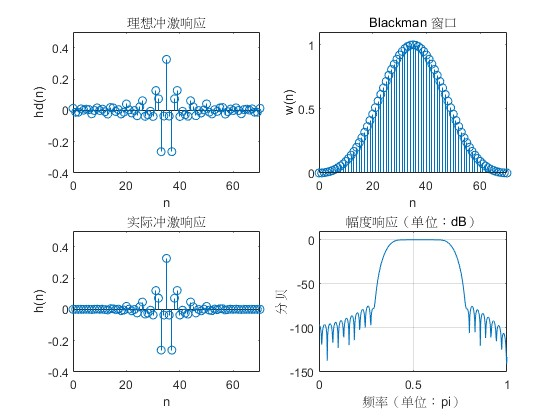
\includegraphics[width=0.8\linewidth]{images/4_Verify/fir.jpg}
\captionof{figure}{窗函数法设计FIR滤波器结果} 
\justifying

在这个FIR滤波器设计的分析中,有以下几个关键变量和步骤:

\begin{itemize}
  \item \texttt{hd(n)}:展示了FIR带阻滤波器的理想冲激响应。理想冲激响应是通过相减两个理想低通滤波器的响应得到的,即
  \[
  \texttt{ideal\_lp(wc2, M) - ideal\_lp(wc1, M)}
  \]
  其中 \texttt{wc1} 和 \texttt{wc2} 是带通滤波器截止频率的中点。

  \item \texttt{w(n)}:理想响应通过与Blackman窗函数相乘,得到实际的冲激响应。Blackman窗是用于减少旁瓣并改善主瓣平滑度的窗函数。

  \item \texttt{h(n)}:实际冲激响应,通过将理想冲激响应和Blackman窗函数相乘得到。

  \item \texttt{db}:显示了滤波器的频率响应,以分贝(dB)表示。图示显示在阻带频率处衰减显著,达到设计要求的40 dB衰减。
\end{itemize}

这种设计方法通过结合理想滤波器响应和窗函数的特性,成功地实现了一个性能优良的FIR带阻滤波器。

\subsubsection{双线性变换法设计IIR滤波器}
代码主要思路如下:

\begin{itemize}
  \item \textbf{初始化和参数设置}:
  \begin{itemize}
    \item \texttt{clear all; clc; close all;}:清除MATLAB环境中的所有变量,清空命令窗口,并关闭所有图形窗口。
    \item \texttt{T = 2;} \texttt{fs = 1/T;}:设置采样周期\texttt{T}为2秒,计算相应的采样频率\texttt{fs}。
  \end{itemize}

  \item \textbf{滤波器设计参数}:
  \begin{itemize}
    \item \texttt{wp = [0.45*pi, 0.65*pi];} \texttt{ws = [0.3*pi, 0.8*pi];}:定义通带和阻带的边界频率(以$\pi$为单位的归一化频率)。
    \item \texttt{Wp = (2/T)*tan(wp/2);} \texttt{Ws = (2/T)*tan(ws/2);}:使用预扭转公式将这些归一化频率转换为模拟频率,以适应模拟滤波器设计。
    \item \texttt{Ap = 1;} \texttt{As = 40;}:分别设置通带最大衰减(1dB)和阻带最小衰减(40dB)。
  \end{itemize}

  \item \textbf{巴特沃斯模拟滤波器设计}:
  \begin{itemize}
    \item 使用\texttt{buttord}函数计算滤波器的最小阶数\texttt{N}和截止频率\texttt{Wc}。
    \item 使用\texttt{butter}函数根据这些参数设计巴特沃斯带阻模拟滤波器,得到其系数\texttt{B}和\texttt{A}。
  \end{itemize}

  \item \textbf{频率响应计算}:
  \begin{itemize}
    \item \texttt{Hs = freqs(B, A, W);}:计算模拟滤波器的频率响应。
    \item \texttt{Hz = freqz(Bz, Az, W);}:使用\texttt{bilinear}转换将模拟滤波器转换为数字滤波器,并计算其频率响应。
  \end{itemize}

  \item \textbf{绘图}:
  \begin{itemize}
    \item 绘制模拟滤波器和数字滤波器的幅值响应,分别为图的左侧和右侧。图表中使用\texttt{grid on}增加了网格线,便于观察频率响应的变化。
  \end{itemize}
\end{itemize}

\begin{lstlisting}
clear all;
clc
close all
T = 2;    
fs = 1/T;      
wp = [0.45*pi,0.65*pi];
ws = [0.3*pi,0.8*pi];
Wp = (2/T)*tan(wp/2); 
Ws = (2/T)*tan(ws/2);
Ap = 1; 
As = 40;

[N ,Wc] = buttord(Wp,Ws,Ap,As,'s');
[B ,A] = butter(N,Wc,'stop','s');
W = linspace(0,pi,400*pi);
Hs = freqs(B,A,W);
[Bz,Az] = bilinear(B,A,fs);
Hz = freqz(Bz,Az,W);
 
figure;
subplot(1,2,1);
plot(W/pi,abs(Hs)); 
xlabel('频率/Hz');ylabel('幅值');title('巴特沃斯模拟滤波器');grid on;
subplot(1,2,2);
plot(W/pi,abs(Hz));  
xlabel('频率/Hz');ylabel('幅值');title('巴特沃斯数字滤波器');grid on;

\end{lstlisting}

\centering 
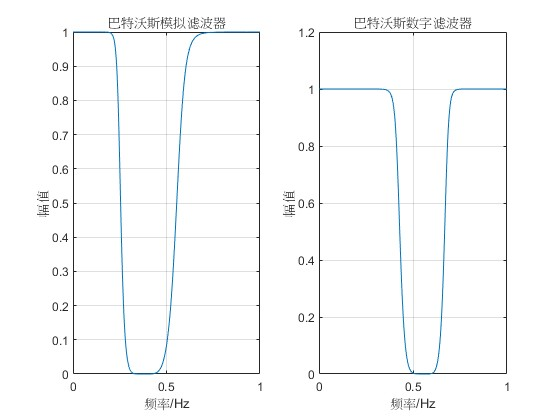
\includegraphics[width=0.8\linewidth]{images/4_Verify/iir.jpg}
\captionof{figure}{双线性变换法设计IIR滤波器结果} 
\justifying


\section{课程设计1(来源实验题目):图像信号的卷积处理}
\subsection{课程设计目的}
\begin{itemize}
    \item 熟悉图像处理常用函数和方法
    \item 培养通过查阅文献解决问题的能力。
    \item 了解图像卷积、卷积核(算子)、常用的卷积核及其用途
\end{itemize}

\subsection{课程设计要求}
\begin{itemize}
    \item \textbf{实现对图像进行不同卷积核的运算:} 可以通过应用不同的卷积核(如锐化、模糊、边缘检测等)来对图像进行滤波处理,改变图像的特征和外观。
    
    \item \textbf{实现图像的加噪、低通滤波、高通滤波、边缘检测、高斯滤波等:} 可以通过添加不同类型的噪声、应用低通、高通、边缘检测和高斯滤波器来改变图像的频域特性和视觉效果。
    
    \item \textbf{对图像进行特效处理:} 可以实现各种图像特效处理,如模糊、马赛克、光照效果、色彩调整等,以增强图像的视觉吸引力和艺术效果。
    
    \item \textbf{对图像进行任意倍数放大和缩小、任意角度旋转:} 可以实现对图像进行缩放和旋转的操作,以改变图像的尺寸和方向,满足不同应用场景下的需求。

    \item \textbf{为程序设计UI图形交互界面}
\end{itemize}



\subsection{课程实验原理}
\subsubsection{图像卷积}
在图像数字信号处理中,卷积是一种常用的操作,用于处理图像以实现各种功能,如图像滤波、特征提取等。卷积操作可以看作是将两个函数(在图像处理中通常是一个图像和一个卷积核)进行加权求和的过程,其中卷积核是一个小的矩阵,用于对图像进行局部区域的加权处理。

给定一个图像 \( I \) 和一个卷积核 \( K \),卷积操作可以用以下公式表示:

\begin{equation}
(I * K)(m, n) = \sum_{i=-\infty}^{\infty} \sum_{j=-\infty}^{\infty} I(i, j) \cdot K(m-i, n-j)
\end{equation}


其中,\( (m, n) \) 表示图像的像素位置,\( I(i, j) \) 表示图像在位置 \( (i, j) \) 处的像素值,\( K(m-i, n-j) \) 表示卷积核在位置 \( (m-i, n-j) \) 处的权重。

卷积操作的过程可以简单描述为:将卷积核与图像的每个像素位置进行对齐,然后将卷积核的每个元素与与之对应的图像像素进行乘法运算,最后将所有乘积结果相加得到输出图像的像素值。

在实际应用中,卷积操作常用于图像滤波,通过选择不同的卷积核可以实现不同的滤波效果,如平滑、锐化、边缘检测等。卷积操作也被广泛用于深度学习中的卷积神经网络(CNN),用于图像分类、目标检测等任务。
\subsubsection{低通滤波器}
低通滤波器是一种常用的图像滤波器,用于去除图像中高频部分,保留图像中的低频信息,从而实现图像的平滑和去噪。低通滤波器通过减小图像中像素值之间的变化来实现平滑效果,常用于图像预处理、去除噪声以及图像恢复等应用场景。

以下是一些常见的低通滤波器及其卷积核的示例:
\begin{itemize}
    \item 均值滤波器: 均值滤波器使用一个固定大小的卷积核,在卷积核的区域内取平均值作为输出像素的值。常见的均值滤波器包括 3x3 和 5x5 的卷积核,示例如下:
    \[
\text{3x3 均值滤波器:} \quad \frac{1}{9} \begin{bmatrix}
1 & 1 & 1 \\
1 & 1 & 1 \\
1 & 1 & 1 \\
\end{bmatrix}
\]

\[
\text{5x5 均值滤波器:} \quad \frac{1}{25} \begin{bmatrix}
1 & 1 & 1 & 1 & 1 \\
1 & 1 & 1 & 1 & 1 \\
1 & 1 & 1 & 1 & 1 \\
1 & 1 & 1 & 1 & 1 \\
1 & 1 & 1 & 1 & 1 \\
\end{bmatrix}
\]

均值滤波器的效果是平滑图像,去除图像中的细节和噪声,但可能会导致图像变得模糊。

    \item 高斯滤波器: 高斯滤波器使用高斯函数作为卷积核,以加权平均的方式对图像进行滤波。高斯滤波器在滤波过程中考虑了像素距离中心像素的距离,使得距离中心更近的像素具有更大的权重。常见的高斯滤波器示例如下:
\[
\text{3x3 高斯滤波器:} \quad \frac{1}{16} \begin{bmatrix}
1 & 2 & 1 \\
2 & 4 & 2 \\
1 & 2 & 1 \\
\end{bmatrix}
\]

\[
\text{5x5 高斯滤波器:} \quad \frac{1}{273} \begin{bmatrix}
1 & 4 & 7 & 4 & 1 \\
4 & 16 & 26 & 16 & 4 \\
7 & 26 & 41 & 26 & 7 \\
4 & 16 & 26 & 16 & 4 \\
1 & 4 & 7 & 4 & 1 \\
\end{bmatrix}
\]

高斯滤波器具有平滑效果,同时保留了图像的细节,不会造成明显的模糊。
    
\end{itemize}

\subsubsection{高通滤波器}
高通滤波器是一种图像处理滤波器,用于增强图像中的高频部分,抑制图像中的低频部分,从而突出图像的边缘和细节特征。高通滤波器通常用于图像锐化、边缘检测等应用场景。

以下是一些常见的高通滤波器及其卷积核的示例:

\begin{itemize}
    \item 拉普拉斯滤波器:拉普拉斯滤波器对图像进行二阶微分,可以提取图像中的边缘和细节信息。常见的拉普拉斯滤波器示例如下:
    
    \begin{itemize}
        \item 3x3 拉普拉斯滤波器:
        \[
        \begin{bmatrix}
        0 & -1 & 0 \\
        -1 & 4 & -1 \\
        0 & -1 & 0 \\
        \end{bmatrix}
        \]
        
        \item 5x5 拉普拉斯滤波器:
        \[
        \begin{bmatrix}
        0 & 0 & -1 & 0 & 0 \\
        0 & -1 & -2 & -1 & 0 \\
        -1 & -2 & 16 & -2 & -1 \\
        0 & -1 & -2 & -1 & 0 \\
        0 & 0 & -1 & 0 & 0 \\
        \end{bmatrix}
        \]
        拉普拉斯滤波器能够增强图像中的边缘和细节,但同时也会增加图像中的噪声。
    \end{itemize}

    \item Sobel 滤波器:Sobel 滤波器是一种常用的边缘检测滤波器,通过计算图像的梯度来识别图像中的边缘。Sobel 滤波器有水平方向和垂直方向两种形式,分别用于检测图像中的水平和垂直边缘。常见的 Sobel 滤波器示例如下:
    \begin{itemize}
        \item 水平方向 Sobel 滤波器:
        \[
        \begin{bmatrix}
        -1 & 0 & 1 \\
        -2 & 0 & 2 \\
        -1 & 0 & 1 \\
        \end{bmatrix}
        \]
        
        \item 垂直方向 Sobel 滤波器:
        \[
        \begin{bmatrix}
        -1 & -2 & -1 \\
        0 & 0 & 0 \\
        1 & 2 & 1 \\
        \end{bmatrix}
        \]
    \end{itemize}

    Sobel 滤波器能够有效地检测图像中的边缘,提取出图像中的细节信息。
\end{itemize}

\subsubsection{匹配滤波边缘}
匹配滤波边缘是一种常用于图像处理中的边缘检测方法。其基本思想是利用模板或滤波器与图像进行卷积,通过与预先定义的边缘模式或特征模式进行匹配,从而识别图像中的边缘或特征。

常见的滤波器包括以下几种:

\begin{itemize}
    \item \textbf{Prewitt 滤波器:}
    \begin{itemize}
        \item 水平方向 Prewitt 滤波器:
        \[
        \begin{bmatrix}
        -1 & 0 & 1 \\
        -1 & 0 & 1 \\
        -1 & 0 & 1 \\
        \end{bmatrix}
        \]
        
        \item 垂直方向 Prewitt 滤波器:
        \[
        \begin{bmatrix}
        -1 & -1 & -1 \\
        0 & 0 & 0 \\
        1 & 1 & 1 \\
        \end{bmatrix}
        \]
    \end{itemize}

    \item \textbf{Roberts 滤波器:}
    \begin{itemize}
        \item Roberts 交叉梯度滤波器:
        \[
        \begin{bmatrix}
        0 & 1 \\
        -1 & 0 \\
        \end{bmatrix}
        \]
        
        \item Roberts 十字梯度滤波器:
        \[
        \begin{bmatrix}
        1 & 0 \\
        0 & -1 \\
        \end{bmatrix}
        \]
    \end{itemize}
\end{itemize}

匹配滤波边缘方法适用于各种图像处理任务,如目标检测、图像分割、特征提取等。通过调整不同的模板或滤波器,可以实现对不同形状、大小和方向的边缘进行有效的检测和提取。


\subsubsection{边缘检测}
边缘检测是图像处理中常用的技术,用于检测图像中的边缘和轮廓。边缘通常是图像中像素灰度值变化较大的地方,表示图像中物体的边界或区域之间的转换。

常见的边缘检测算法基于卷积操作,通过在图像上应用特定的卷积核来检测边缘。以下是一些常见的边缘检测卷积核及其效果:

    \begin{itemize}
        \item \textbf{Sobel 滤波器:}
        \begin{itemize}
            \item 水平方向 Sobel 滤波器:
            
            \[
            \begin{bmatrix}
            -1 & 0 & 1 \\
            -2 & 0 & 2 \\
            -1 & 0 & 1 \\
            \end{bmatrix}
            \]
            
            \item 垂直方向 Sobel 滤波器:
            
            \[
            \begin{bmatrix}
            -1 & -2 & -1 \\
            0 & 0 & 0 \\
            1 & 2 & 1 \\
            \end{bmatrix}
            \]
        \end{itemize}
        
        \item \textbf{Prewitt 滤波器:}
        \begin{itemize}
            \item 水平方向 Prewitt 滤波器:
            
            \[
            \begin{bmatrix}
            -1 & 0 & 1 \\
            -1 & 0 & 1 \\
            -1 & 0 & 1 \\
            \end{bmatrix}
            \]
            
            \item 垂直方向 Prewitt 滤波器:
            
            \[
            \begin{bmatrix}
            -1 & -1 & -1 \\
            0 & 0 & 0 \\
            1 & 1 & 1 \\
            \end{bmatrix}
            \]
        \end{itemize}
        
        \item Roberts 滤波器:
        \begin{itemize}
            \item Roberts 十字梯度滤波器:
            
            \[
            \begin{bmatrix}
            1 & 0 \\
            0 & -1 \\
            \end{bmatrix}
            \]
            
            \item Roberts 交叉梯度滤波器:
            
            \[
            \begin{bmatrix}
            0 & 1 \\
            -1 & 0 \\
            \end{bmatrix}
            \]
        \end{itemize}
    \end{itemize}


\subsection{课程设计内容}
\subsubsection{图像进行不同卷积核运算}
根据实验要求,常用卷积核(算子、模板)如下图所示:

\centering 
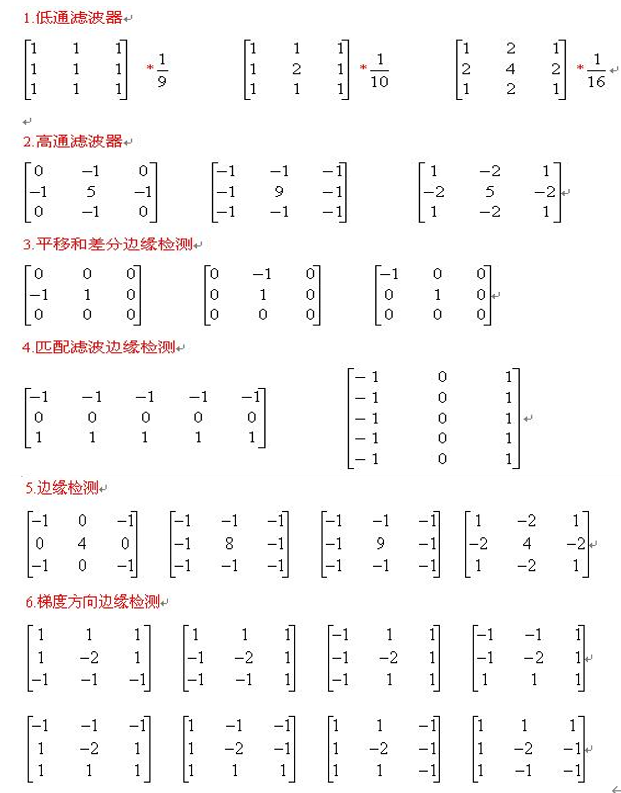
\includegraphics[width=0.8\linewidth]{images/Design/image_processing/all_kernels.png}
\captionof{figure}{常用卷积核(算子、模板)} 
\justifying

处理的图片如下图:

按照上述模板,可以编写出以下代码:
\begin{lstlisting}[style=python]
import cv2
import numpy as np

# 例如,这是一个使用卷积核1的函数
def kernel_lowpass_1(image):
    kernel = np.array([[1, 1, 1],
                       [1, 1, 1],
                       [1, 1, 1]]) / 9
    return cv2.filter2D(image, -1, kernel)

def kernel_lowpass_2(image):
    kernel = np.array([[1, 1, 1],
                       [1, 2, 1],
                       [1, 1, 1]]) / 10
    return cv2.filter2D(image, -1, kernel)

def kernel_lowpass_3(image):
    kernel = np.array([[1, 2, 1],
                       [2, 4, 2],
                       [1, 2, 1]]) / 16
    return cv2.filter2D(image, -1, kernel)

def kernel_highpass_1(image):
    kernel = np.array([[0, -1, 0],
                       [-1, 5, -1],
                       [0, -1, 0]])
    return cv2.filter2D(image, -1, kernel)

def kernel_highpass_2(image):
    kernel = np.array([[-1, -1, -1],
                       [-1, 9, -1],
                       [-1, -1, -1]])
    return cv2.filter2D(image, -1, kernel)

def kernel_highpass_3(image):
    kernel = np.array([[1, -2, 1],
                       [-2, 5, -2],
                       [1, -2, 1]])
    return cv2.filter2D(image, -1, kernel)

def kernel_move_detection_horizontal(image):
    kernel = np.array([[0, 0, 0],
                       [-1, 1, 0],
                       [0, 0, 0]])
    return cv2.filter2D(image, -1, kernel)

def kernel_move_detection_vertical(image):
    kernel = np.array([[0, -1, 0],
                       [0, 1, 0],
                       [0, 0, 0]])
    return cv2.filter2D(image, -1, kernel)

def kernel_move_detection_diagonal(image):
    kernel = np.array([[-1, 0, 0],
                       [0, 1, 0],
                       [0, 0, 0]])
    return cv2.filter2D(image, -1, kernel)

def kernel_horizontal_match_detection(image):
    kernel = np.array([[-1, -1, -1, -1, -1],
                       [0, 0, 0, 0, 0],
                       [1, 1, 1, 1, 1]])
    return cv2.filter2D(image, -1, kernel)

def kernel_vertical_match_detection(image):
    kernel = np.array([[-1, 0, 1],
                       [-1, 0, 1],
                       [-1, 0, 1]])
    return cv2.filter2D(image, -1, kernel)

def kernel_edge_1(image):
    kernel = np.array([[-1, 0, -1],
                       [0, 4, 0],
                       [-1, 0, -1]])
    return cv2.filter2D(image, -1, kernel)

def kernel_edge_2(image):
    kernel = np.array([[-1, -1, -1],
                       [-1, 8, -1],
                       [-1, -1, -1]])
    return cv2.filter2D(image, -1, kernel)

def kernel_edge_3(image):
    kernel = np.array([[-1, -1, -1],
                       [-1, 9, -1],
                       [-1, -1, -1]])
    return cv2.filter2D(image, -1, kernel)

def kernel_edge_4(image):
    kernel = np.array([[1, -2, 1],
                       [-2, 4, -2],
                       [1, -2, 1]])
    return cv2.filter2D(image, -1, kernel)

def kernel_gradient_1(image):
    kernel = np.array([[1, 1, 1],
                       [1, -2, 1],
                       [-1, -1, -1]])
    return cv2.filter2D(image, -1, kernel)

def kernel_gradient_2(image):
    kernel = np.array([[1, 1, 1],
                       [-1, -2, 1],
                       [-1, -1, 1]])
    return cv2.filter2D(image, -1, kernel)

def kernel_gradient_3(image):
    kernel = np.array([[-1, 1, 1],
                       [-1, -2, 1],
                       [-1, 1, 1]])
    return cv2.filter2D(image, -1, kernel)

def kernel_gradient_4(image):
    kernel = np.array([[-1, -1, 1],
                       [-1, -2, 1],
                       [1, 1, 1]])
    return cv2.filter2D(image, -1, kernel)

def kernel_gradient_5(image):
    kernel = np.array([[-1, -1, -1],
                       [1, -2, 1],
                       [1, 1, 1]])
    return cv2.filter2D(image, -1, kernel)

def kernel_gradient_6(image):
    kernel = np.array([[1, -1, -1],
                       [1, -2, -1],
                       [1, 1, 1]])
    return cv2.filter2D(image, -1, kernel)

def kernel_gradient_7(image):
    kernel = np.array([[1, 1, -1],
                       [1, -2, -1],
                       [1, 1, -1]])
    return cv2.filter2D(image, -1, kernel)

def kernel_gradient_8(image):
    kernel = np.array([[1, 1, 1],
                       [1, -2, -1],
                       [1, -1, -1]])
    return cv2.filter2D(image, -1, kernel)
\end{lstlisting}

得到结果如下:
\begin{figure}[h!]
    \centering
    \begin{minipage}[b]{0.48\textwidth}
        \centering
        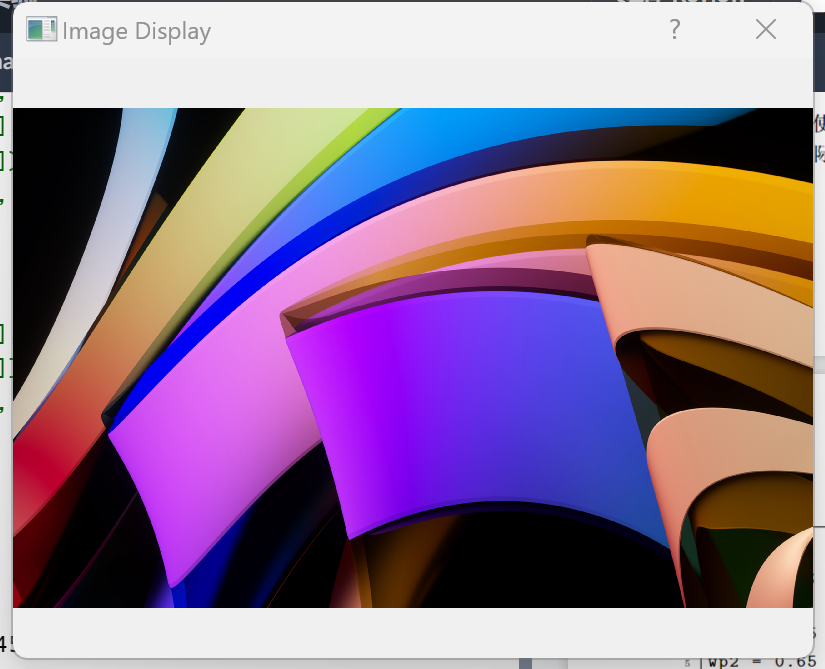
\includegraphics[width=\linewidth]{images/Design/image_processing/1/lowpass.png}
        \caption{低通滤波器算子得到结果}
    \end{minipage}
    \hfill
    \begin{minipage}[b]{0.48\textwidth}
        \centering
        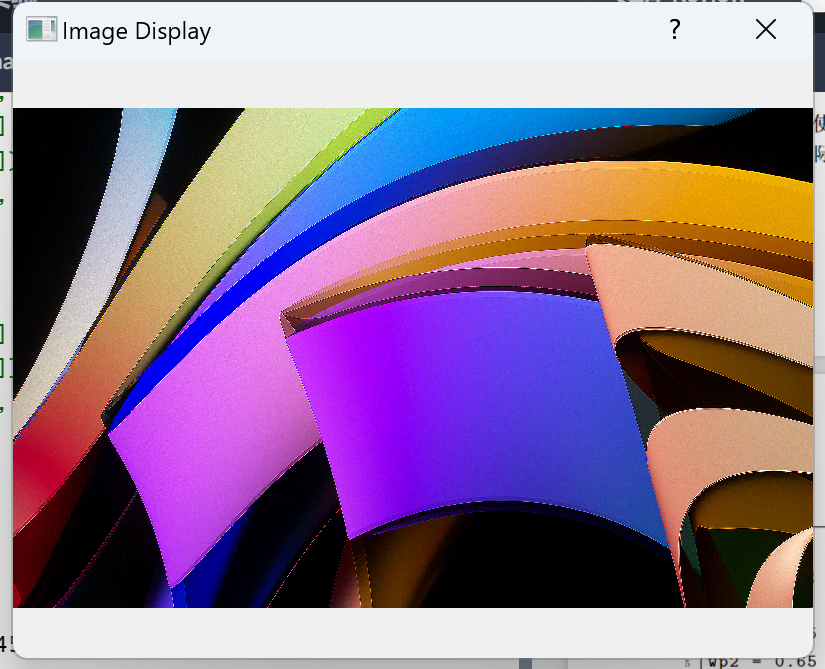
\includegraphics[width=\linewidth]{images/Design/image_processing/1/highpass.png}
        \caption{高通滤波器算子得到结果}
    \end{minipage}
    
    \vspace{0.2cm}
    
    \begin{minipage}[b]{0.48\textwidth}
        \centering
        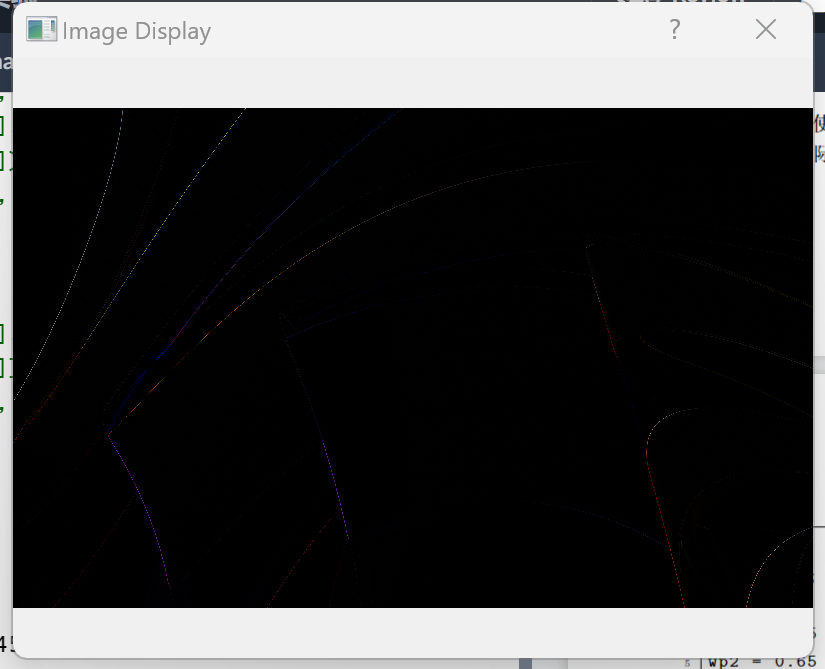
\includegraphics[width=\linewidth]{images/Design/image_processing/1/horizontal.png}
        \caption{水平边缘检测算子得到结果}
    \end{minipage}
    \hfill
    \begin{minipage}[b]{0.48\textwidth}
        \centering
        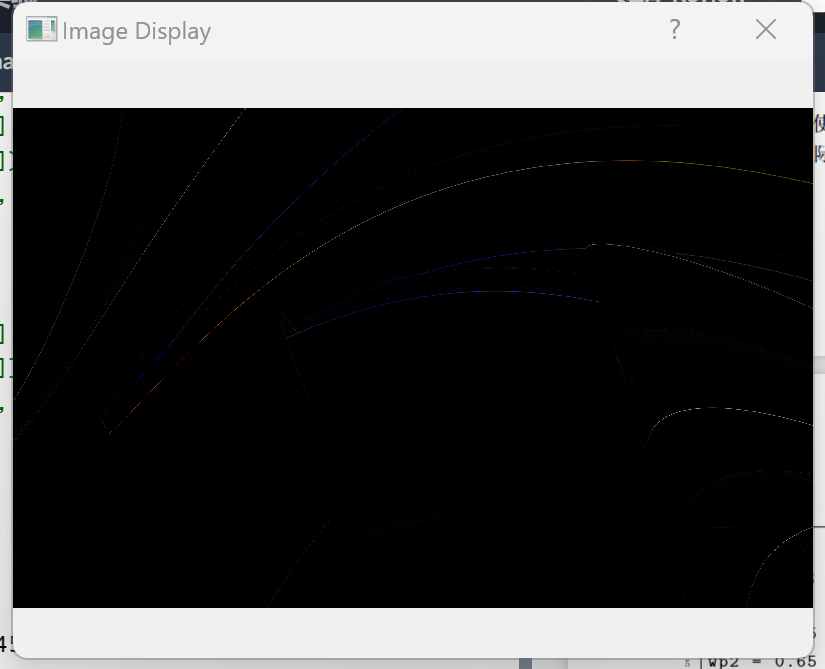
\includegraphics[width=\linewidth]{images/Design/image_processing/1/vertical.png}
        \caption{竖直边缘检测算子得到结果}
    \end{minipage}
\end{figure}
低通滤波器保留了图像中的低频信息,滤除了高频细节。图像看起来更加平滑,边缘细节被模糊化,适用于去除噪声和平滑图像。高通滤波器保留了图像中的高频信息,滤除了低频成分。图像的边缘和细节变得更加明显,但可能会引入噪声,适用于边缘检测和锐化图像。水平边缘检测算子主要检测水平方向上的边缘。图像中水平变化的部分被强调出来,而其他方向的边缘信息较弱。竖直边缘检测算子主要检测竖直方向上的边缘。图像中竖直变化的部分被强调出来,而其他方向的边缘信息较弱。
\begin{figure}[htbp]
    \centering
    \begin{minipage}[b]{0.48\textwidth}
        \centering
        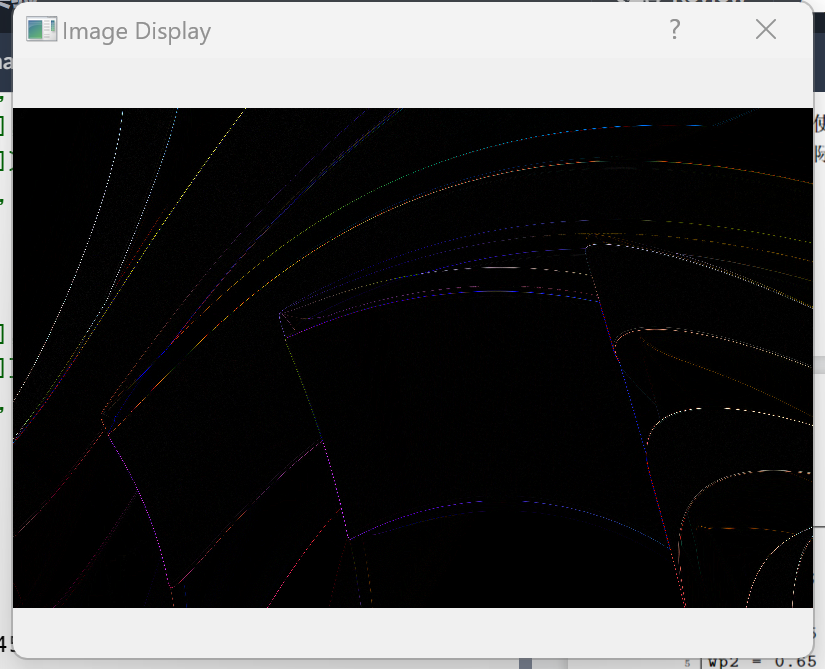
\includegraphics[width=\linewidth]{images/Design/image_processing/1/edge_1.png}
        \caption{边缘检测算子1得到结果}
    \end{minipage}
    \hfill
    \begin{minipage}[b]{0.48\textwidth}
        \centering
        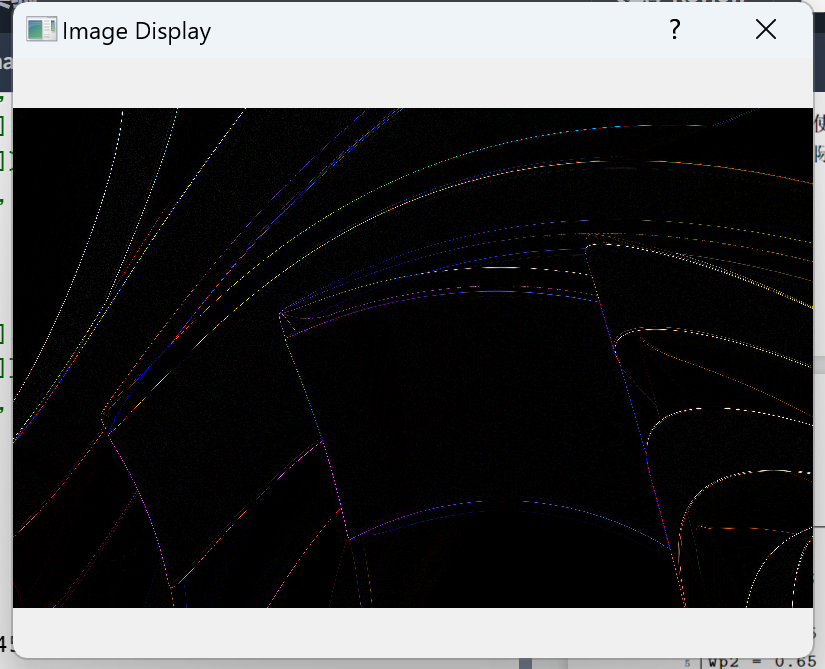
\includegraphics[width=\linewidth]{images/Design/image_processing/1/edge_2.png}
        \caption{边缘检测算子2得到结果}
    \end{minipage}
    
    \vspace{0.2cm}
    
    \begin{minipage}[b]{0.48\textwidth}
        \centering
        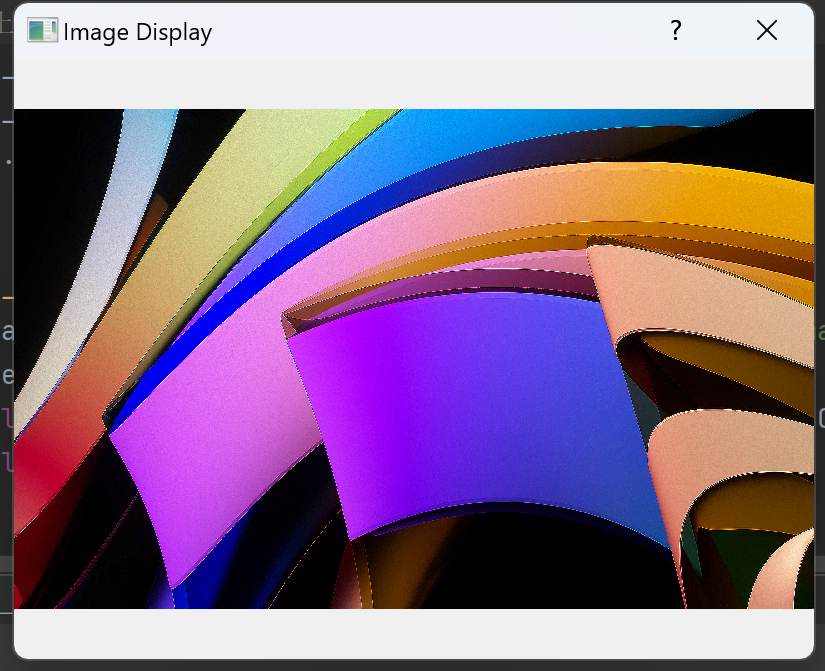
\includegraphics[width=\linewidth]{images/Design/image_processing/1/edge_3.png}
        \caption{边缘检测算子3得到结果}
    \end{minipage}
    \hfill
    \begin{minipage}[b]{0.48\textwidth}
        \centering
        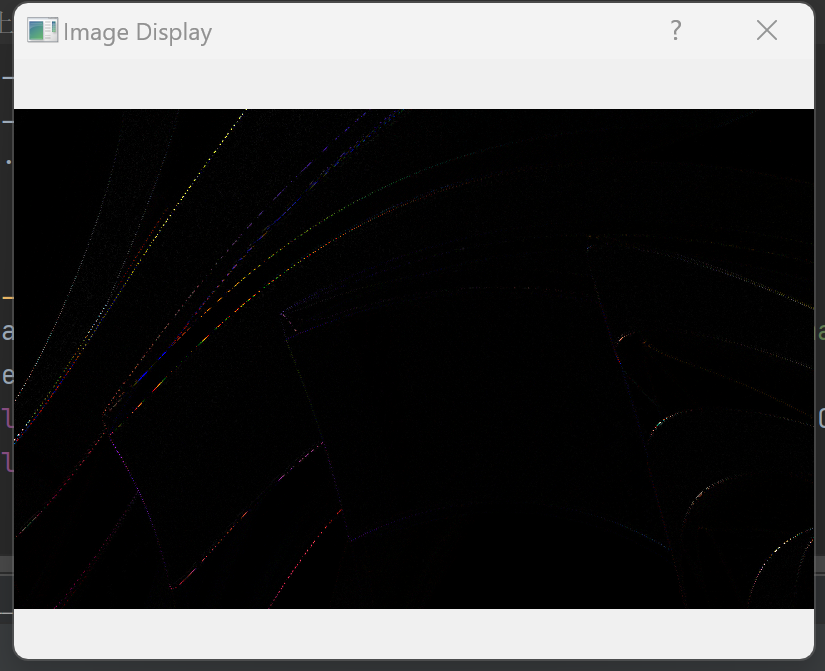
\includegraphics[width=\linewidth]{images/Design/image_processing/1/edge_4.png}
        \caption{边缘检测算子4得到结果}
    \end{minipage}
\end{figure}

\begin{figure}[htbp]
    \centering
    \begin{minipage}[b]{0.48\textwidth}
        \centering
        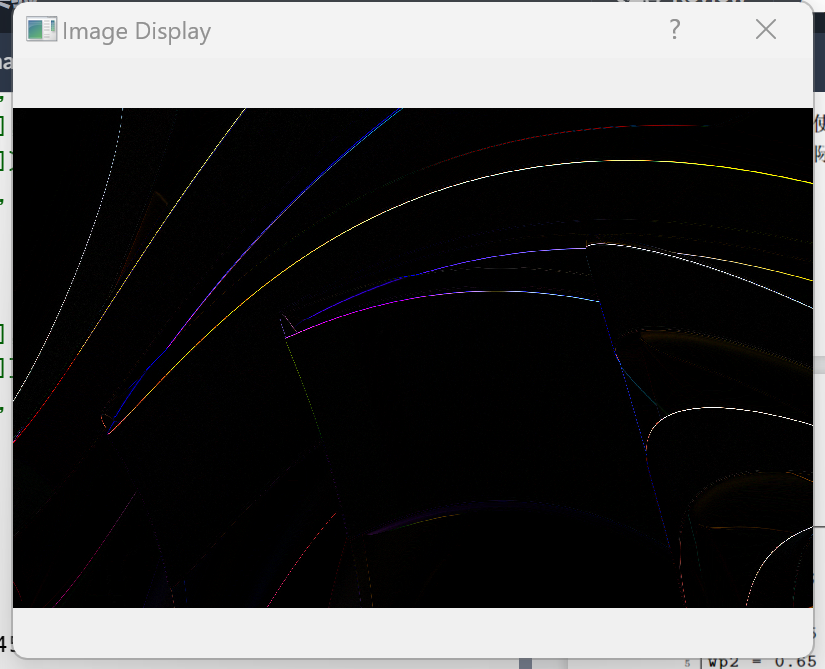
\includegraphics[width=\linewidth]{images/Design/image_processing/1/gradient5.png}
        \caption{梯度方向边缘检测算子1得到结果}
    \end{minipage}
    \hfill
    \begin{minipage}[b]{0.48\textwidth}
        \centering
        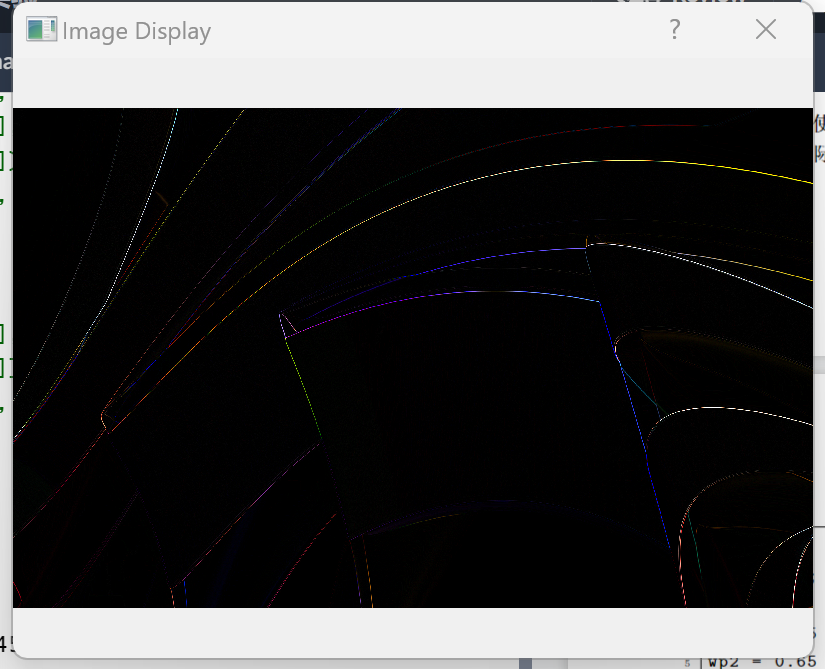
\includegraphics[width=\linewidth]{images/Design/image_processing/1/gradient6.png}
        \caption{梯度方向边缘检测算子2得到结果}
    \end{minipage}
    
    \vspace{0.2cm}
    
    \begin{minipage}[b]{0.48\textwidth}
        \centering
        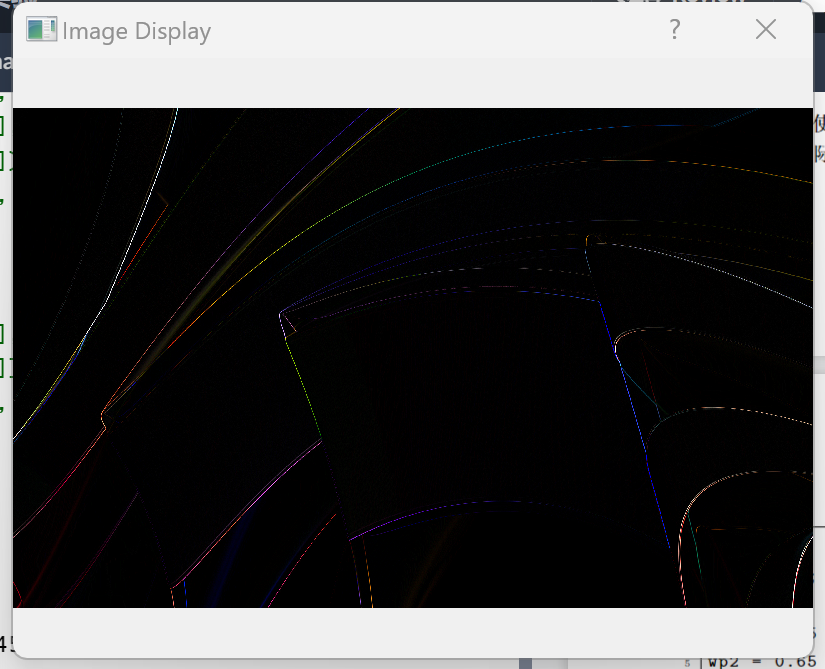
\includegraphics[width=\linewidth]{images/Design/image_processing/1/gradient7.png}
        \caption{梯度方向边缘检测算子3得到结果}
    \end{minipage}
    \hfill
    \begin{minipage}[b]{0.48\textwidth}
        \centering
        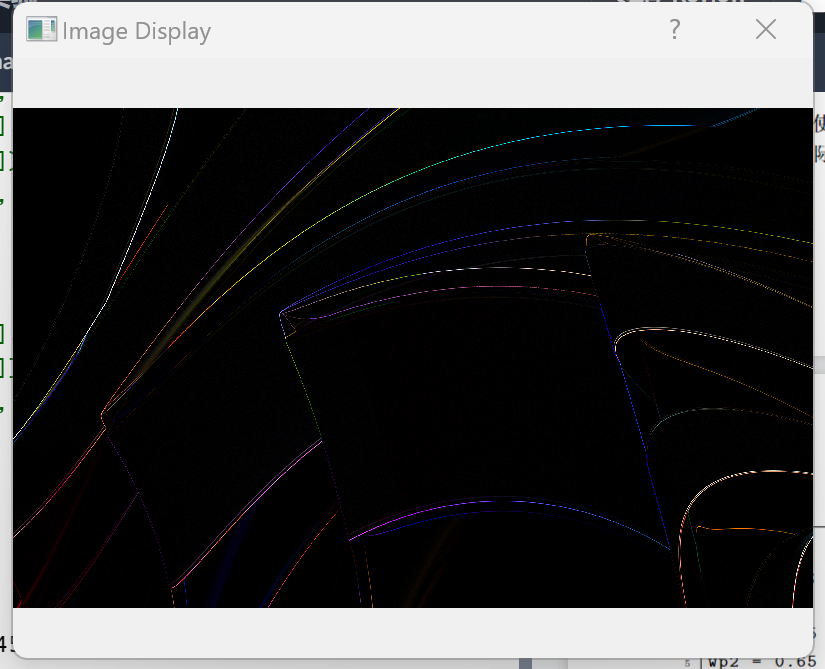
\includegraphics[width=\linewidth]{images/Design/image_processing/1/gradient8.png}
        \caption{梯度方向边缘检测算子4得到结果}
    \end{minipage}
\end{figure}


\clearpage
\subsubsection{图像基本处理}
图像的基本处理包括以下几个内容:
\begin{itemize}
    \item 增加高斯噪音、椒盐噪声、泊松噪声
    \item 运用低通滤波、高通滤波
    \item 检测图像边缘(Canny算法)
    \item 加入高斯模糊、中值模糊
    \item 锐化图片
    \item 增强对比度
\end{itemize}

根据上述描述,可以得到以下代码:
\begin{lstlisting}[style=python]
import cv2
import numpy as np

def add_gaussian_noise(image, mean=0, var=0.01):
    row, col, ch = image.shape
    sigma = var ** 0.5
    gauss = np.random.normal(mean, sigma, (row, col, ch))
    noisy = image + gauss.reshape(row, col, ch)
    return np.clip(noisy, 0, 255).astype(np.uint8)

def add_salt_and_pepper_noise(image, s_vs_p=0.5, amount=0.004):
    row, col, ch = image.shape
    out = np.copy(image)
    # Salt mode
    num_salt = np.ceil(amount * image.size * s_vs_p)
    coords = [np.random.randint(0, i - 1, int(num_salt))
              for i in image.shape]
    out[tuple(coords)] = 1

    # Pepper mode
    num_pepper = np.ceil(amount * image.size * (1. - s_vs_p))
    coords = [np.random.randint(0, i - 1, int(num_pepper))
              for i in image.shape]
    out[tuple(coords)] = 0
    return out

def add_poisson_noise(image):
    vals = len(np.unique(image))
    vals = 2 ** np.ceil(np.log2(vals))
    noisy = np.random.poisson(image * vals) / float(vals)
    return np.clip(noisy, 0, 255).astype(np.uint8)


def apply_low_pass_filter(image):
    kernel = np.ones((5, 5), np.float32) / 25
    return cv2.filter2D(image, -1, kernel)

def apply_high_pass_filter(image):
    kernel = np.array([[0, -1, 0],
                       [-1, 4, -1],
                       [0, -1, 0]])
    return cv2.filter2D(image, -1, kernel)

def detect_edges(image):
    # 使用 Canny 算法检测边缘
    edges = cv2.Canny(image, 100, 200)
    # 创建一个彩色图像用于显示边缘
    edge_colored = cv2.cvtColor(edges, cv2.COLOR_GRAY2BGR)
    return edge_colored


def apply_gaussian_blur(image, ksize=5):
    # 高斯模糊
    return cv2.GaussianBlur(image, (ksize, ksize), 0)

def sharpen_image(image):
    kernel = np.array([[-1, -1, -1],
                       [-1, 9, -1],
                       [-1, -1, -1]])
    return cv2.filter2D(image, -1, kernel)

def apply_median_blur(image, ksize=5):
    # 中值模糊
    return cv2.medianBlur(image, ksize)

def adjust_contrast(image, contrast=1.5):
    # 增强对比度
    f = 131 * (contrast - 1)
    alpha_c = f / 127 + 1
    gamma_c = 127 * (1 - alpha_c)
    image = cv2.addWeighted(image, alpha_c, image, 0, gamma_c)
    return image
\end{lstlisting}

得到的结果如下图所示:

\begin{figure}[htbp]
    \centering
    \begin{minipage}[b]{0.48\textwidth}
        \centering
        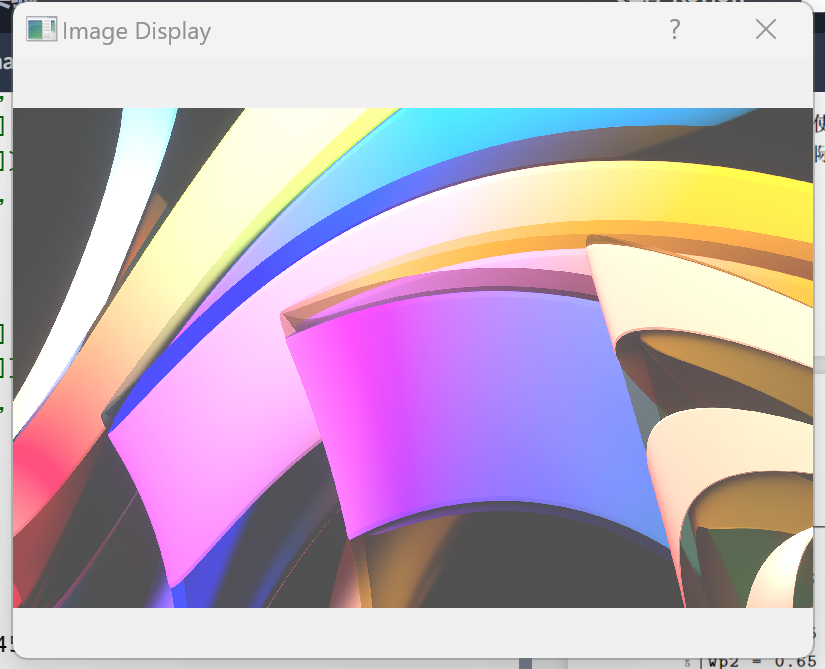
\includegraphics[width=\linewidth]{images/Design/image_processing/2/gaussian_noise.png}
        \caption{高斯噪音得到结果}
    \end{minipage}
    \hfill
    \begin{minipage}[b]{0.48\textwidth}
        \centering
        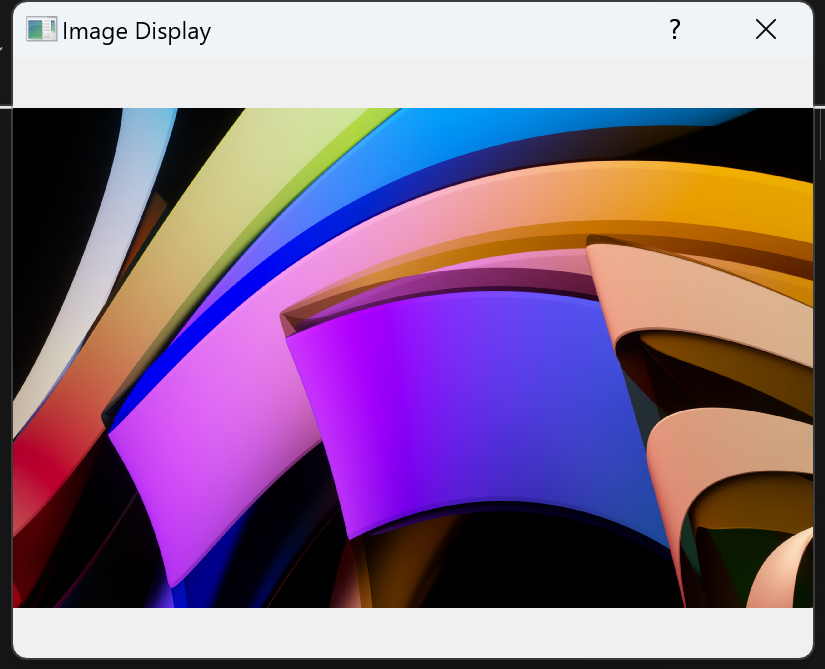
\includegraphics[width=\linewidth]{images/Design/image_processing/2/gaussian_blur.png}
        \caption{高斯模糊得到结果}
    \end{minipage}
    
    \vspace{0.2cm}
    
    \begin{minipage}[b]{0.48\textwidth}
        \centering
        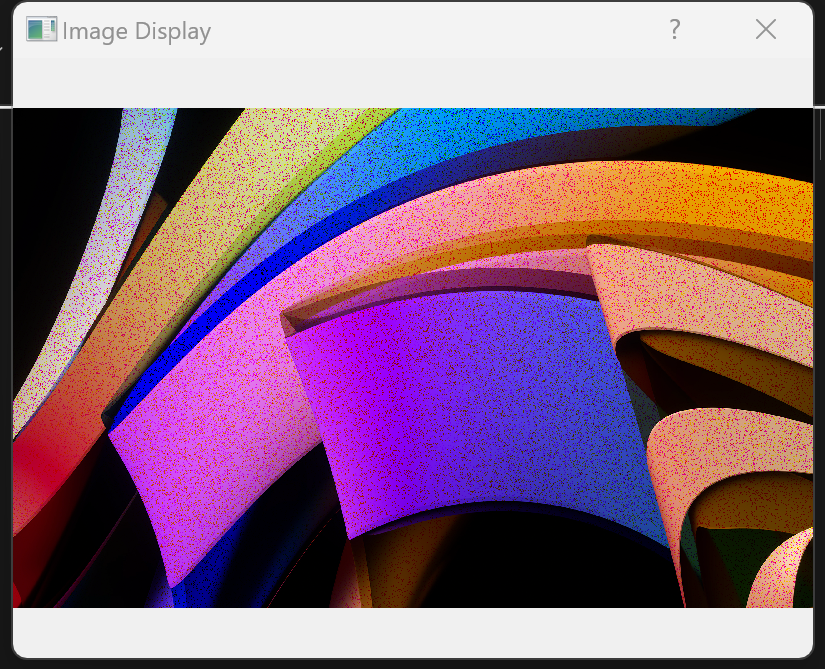
\includegraphics[width=\linewidth]{images/Design/image_processing/2/pepper_noise.png}
        \caption{椒盐噪声得到结果}
    \end{minipage}
    \hfill
    \begin{minipage}[b]{0.48\textwidth}
        \centering
        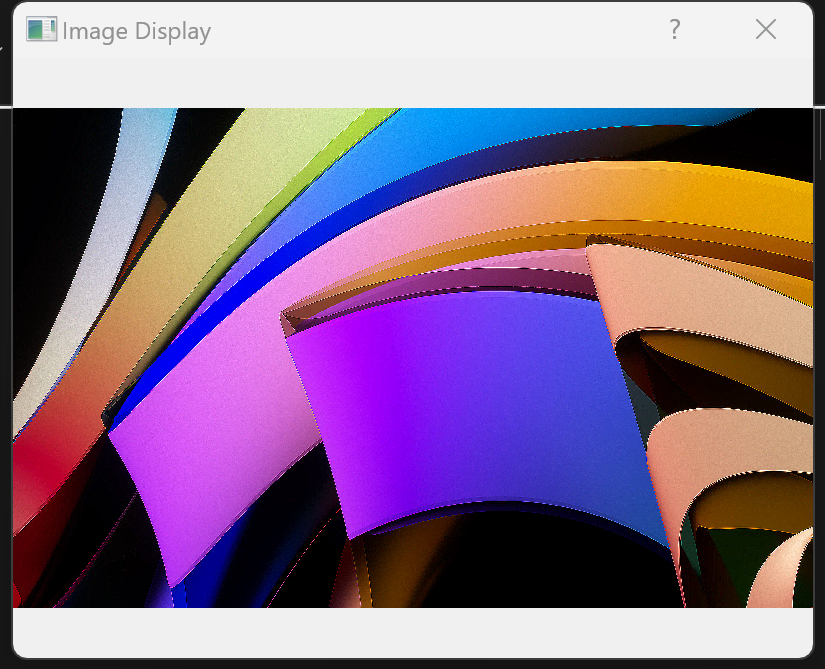
\includegraphics[width=\linewidth]{images/Design/image_processing/2/sharpen.png}
        \caption{锐化处理得到结果}
    \end{minipage}

    \vspace{0.2cm}
    \begin{minipage}[b]{0.48\textwidth}
        \centering
        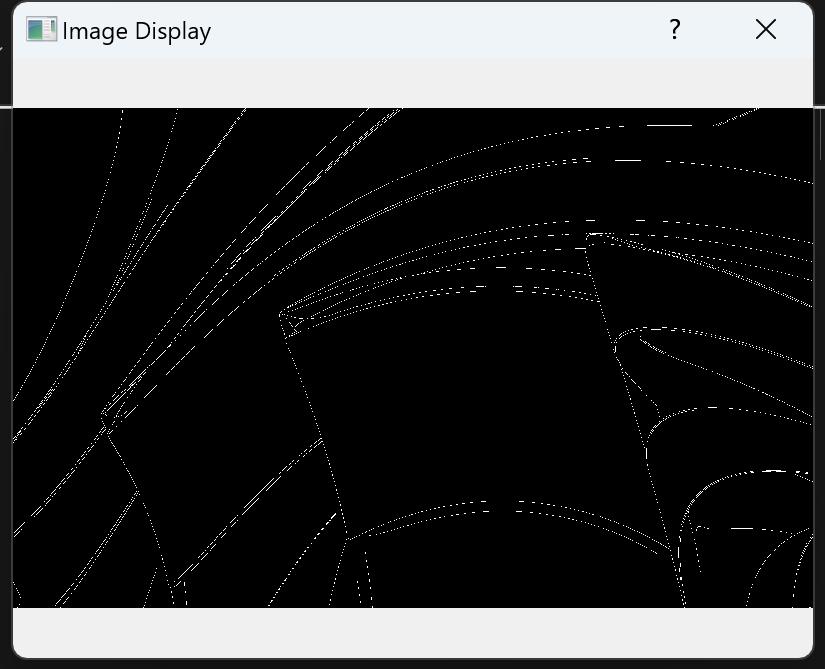
\includegraphics[width=\linewidth]{images/Design/image_processing/2/detect_edges.png}
        \caption{边缘检测得到结果}
    \end{minipage}
    \hfill
    \begin{minipage}[b]{0.48\textwidth}
        \centering
        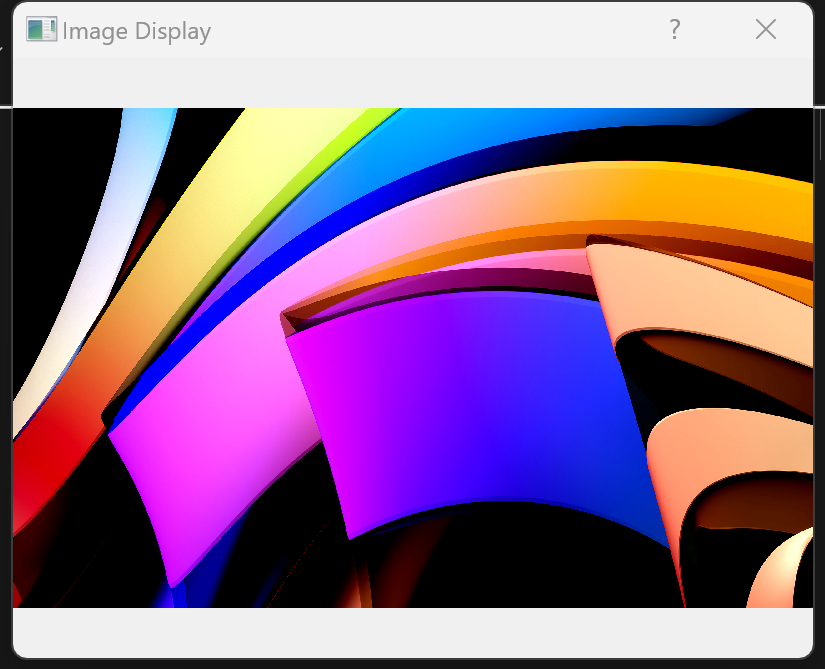
\includegraphics[width=\linewidth]{images/Design/image_processing/2/adjust_contrast.png}
        \caption{增强对比度得到结果}
    \end{minipage}
\end{figure}

图16中的高斯噪音处理在图像中引入了随机分布的亮度变化,使图像显得较为“脏”,模拟了图像传感器的噪音情况。图17的高斯模糊对图像进行了平滑处理,使边缘和细节变得模糊,效果自然和平滑。图18的椒盐噪声处理在图像中引入了随机分布的黑白点,用于模拟图像传输过程中产生的噪声。图19中的锐化处理使图像的边缘和细节更加清晰,整体对比度有所提高,但过度锐化可能会引入噪声。图20的边缘检测算子提取了图像中的边缘信息,结果图像仅显示边缘轮廓,其他部分变为黑色,这些边缘检测算法包括Sobel、Prewitt和Canny等,通过计算图像梯度找到边缘位置。图21的增强对比度处理使图像的亮部更亮,暗部更暗,从而提高图像的对比度,使图像更鲜明和有层次感,但过度处理可能会丢失部分细节。这些处理方法展示了不同算法在图像分析和计算机视觉中的广泛应用,噪声和模糊处理展示了图像在传输和采集过程中可能遇到的干扰,而锐化和对比度增强则是常用的图像增强技术,边缘检测则用于提取图像的轮廓信息。

\clearpage
\subsubsection{图像特效处理}
图像的基本处理包括以下几个内容:
\begin{itemize}
    \item 马赛克处理
    \item 运用低通滤波、高通滤波
    \item 检测图像边缘(Canny算法)
    \item 加入高斯模糊、中值模糊
    \item 锐化图片
    \item 增强对比度
\end{itemize}

\begin{lstlisting}[style=python]
import cv2
import numpy as np

def apply_mosaic(image, block_size=10):
    """
    Apply a mosaic (pixelation) effect to the image.
    :param image: Input image
    :param block_size: Size of each block
    :return: Image with mosaic effect
    """
    for i in range(0, image.shape[0], block_size):
        for j in range(0, image.shape[1], block_size):
            image[i:i+block_size, j:j+block_size] = np.median(image[i:i+block_size, j:j+block_size], axis=(0, 1)).astype(np.uint8)
    return image

def apply_vignette(image, strength=0.5):
    """
    Apply a vignette effect to the image.
    :param image: Input image
    :param strength: Strength of the vignette effect
    :return: Image with vignette effect
    """
    rows, cols = image.shape[:2]
    kernel_x = cv2.getGaussianKernel(cols, cols * strength)
    kernel_y = cv2.getGaussianKernel(rows, rows * strength)
    kernel = kernel_y * kernel_x.T
    mask = 255 * kernel / np.linalg.norm(kernel)
    mask = mask.astype(np.uint8)
    vignette = np.dstack([mask] * 3)
    return cv2.addWeighted(image, 1, vignette, -1, 0)

def apply_thermal_effect(image):
    """
    Simulate a thermal camera effect.
    :param image: Input image
    :return: Image with thermal effect
    """
    gray = cv2.cvtColor(image, cv2.COLOR_BGR2GRAY)
    heatmap = cv2.applyColorMap(gray, cv2.COLORMAP_JET)
    return heatmap

def apply_sketch_effect(image, sigma_s=60, sigma_r=0.07):
    """
    Convert an image to a sketch-like effect using edge-preserving filtering.
    :param image: Input image
    :param sigma_s: Range between 0 and 200.
    :param sigma_r: Range between 0 and 1.
    :return: Sketch-like effect image
    """
    return cv2.stylization(image, sigma_s=sigma_s, sigma_r=sigma_r)

def apply_cartoon_effect(image):
    """
    Apply a cartoon effect to an image.
    :param image: Input image
    :return: Cartoon-styled image
    """
    # Use bilateral filter for edge-aware smoothing.
    smooth = cv2.bilateralFilter(image, d=9, sigmaColor=75, sigmaSpace=75)
    # Convert to grayscale and apply median blur
    gray = cv2.cvtColor(smooth, cv2.COLOR_BGR2GRAY)
    gray = cv2.medianBlur(gray, 7)
    # Detect edges and enhance them
    edges = cv2.adaptiveThreshold(gray, 255, cv2.ADAPTIVE_THRESH_MEAN_C, cv2.THRESH_BINARY, blockSize=9, C=2)
    # Combine the edges and the smoothed image
    cartoon = cv2.bitwise_and(smooth, smooth, mask=edges)
    return cartoon


\end{lstlisting}

得到的结果如下图:
\begin{figure}[h!]
    \centering
    \begin{minipage}[b]{0.48\textwidth}
        \centering
        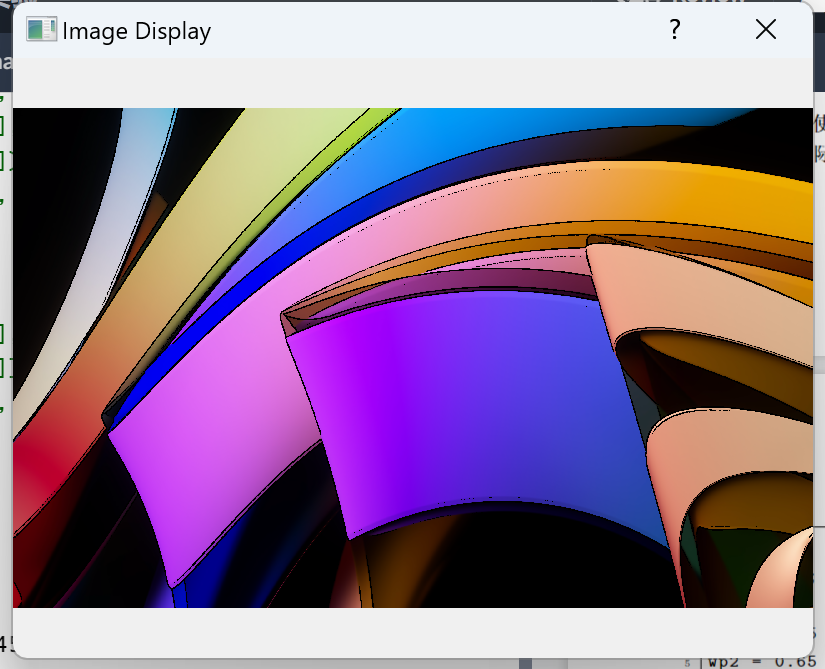
\includegraphics[width=\linewidth]{images/Design/image_processing/3/carton.png}
        \caption{图像卡通化处理得到结果}
    \end{minipage}
    \hfill
    \begin{minipage}[b]{0.48\textwidth}
        \centering
        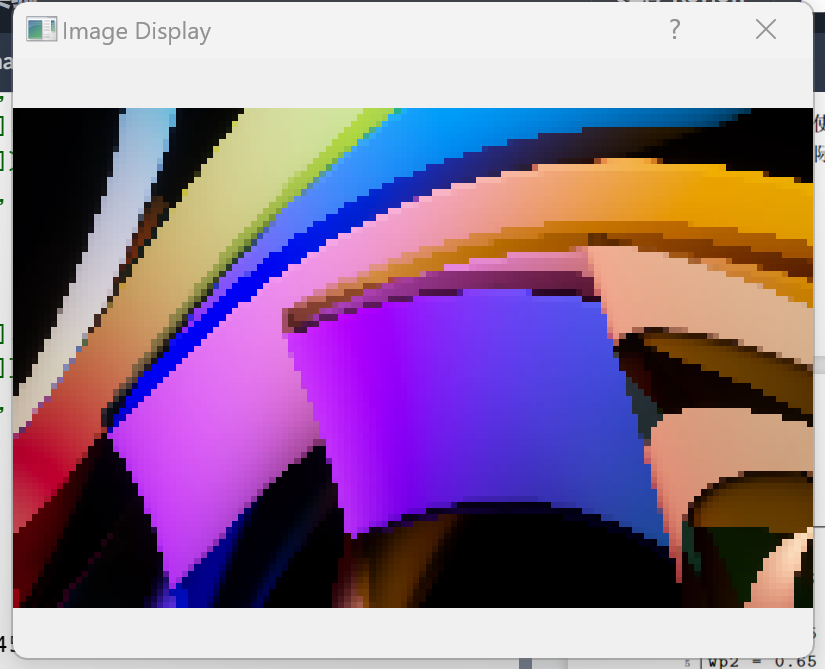
\includegraphics[width=\linewidth]{images/Design/image_processing/3/mosaic.png}
        \caption{图像马赛克处理得到结果}
    \end{minipage}
    
    \vspace{0.2cm}
    
    \begin{minipage}[b]{0.48\textwidth}
        \centering
        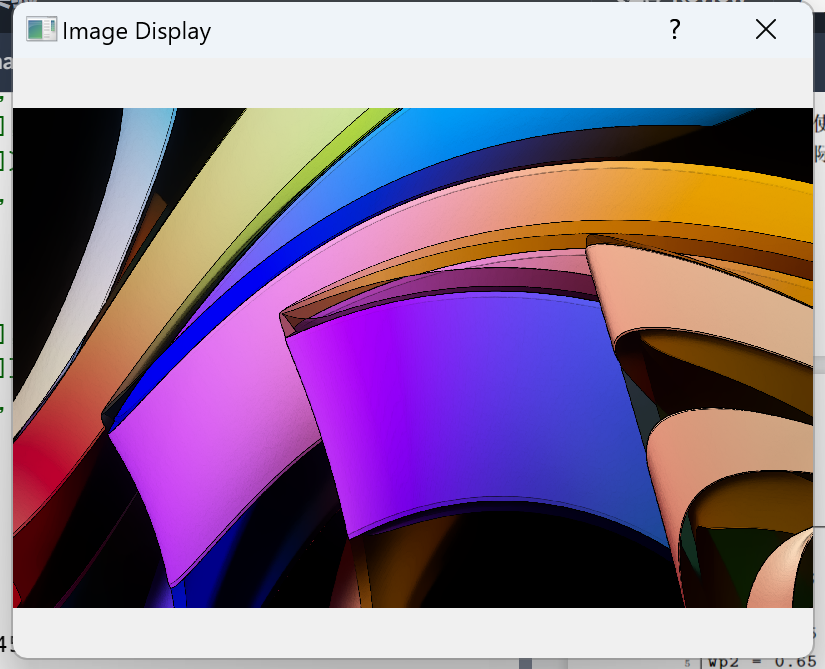
\includegraphics[width=\linewidth]{images/Design/image_processing/3/sketch.png}
        \caption{图像素描化处理得到结果}
    \end{minipage}
    \hfill
    \begin{minipage}[b]{0.48\textwidth}
        \centering
        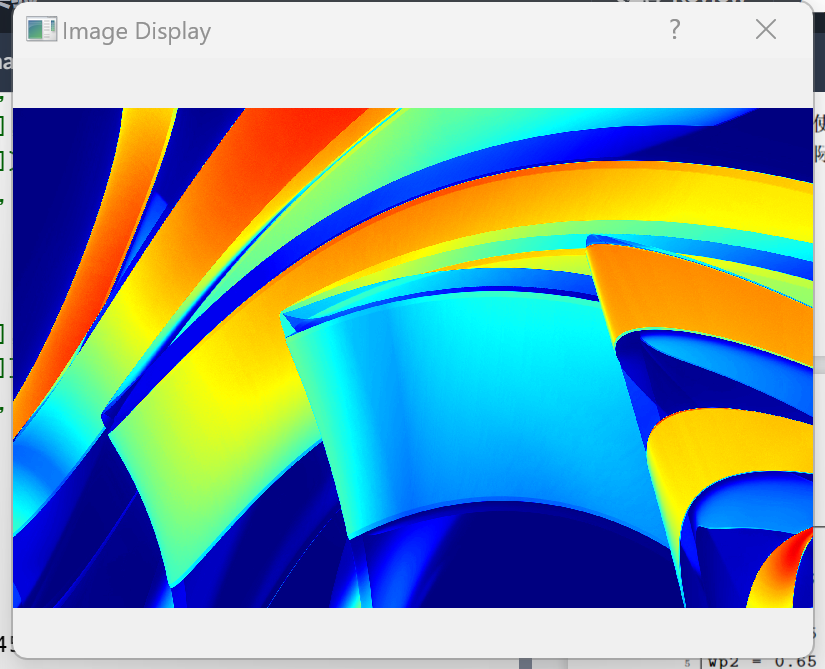
\includegraphics[width=\linewidth]{images/Design/image_processing/3/thermal.png}
        \caption{图像热度图处理得到结果}
    \end{minipage}
\end{figure}

图22展示了图像卡通化处理的结果,该处理通过减少颜色数量和强调边缘,使图像看起来像卡通图。图23中的图像马赛克处理使图像被分割成小块,每块内的像素值相同,类似于隐私保护的模糊效果。图24的图像素描化处理将图像转化为黑白素描效果,保留了主要的边缘和轮廓,使其看起来像手绘素描。图25的图像热度图处理将图像的颜色映射到热度图上,用不同颜色表示不同的强度值,从而突出图像中的强度变化。这些处理方法展示了图像处理的多种技术,卡通化和素描化处理常用于艺术效果和滤镜,马赛克处理用于隐私保护,而热度图处理则用于数据可视化和分析。

\clearpage
\subsubsection{图像变换处理}
图像变换处理包括以下两个内容:
\begin{itemize}
    \item 图像任意倍数放大缩小
    \item 图像任意角度旋转
\end{itemize}
根据上述描述,可以得到以下代码:
\begin{lstlisting}[style=python]
import cv2
import numpy as np


def resize_image(image, scale_factor):
    """
    Resize an image by a given scale factor.
    :param image: Input image.
    :param scale_factor: Scale factor for resizing, e.g., 2 for doubling the size, 0.5 for halving.
    :return: Resized image.
    """
    new_dimensions = (int(image.shape[1] * scale_factor), int(image.shape[0] * scale_factor))
    resized_image = cv2.resize(image, new_dimensions, interpolation=cv2.INTER_LINEAR)
    return resized_image


def rotate_image(image, angle, scale=1.0):
    """
    Rotate an image by a given angle.
    :param image: Input image.
    :param angle: Angle in degrees to rotate the image. Positive values mean counter-clockwise rotation.
    :param scale: Scale factor during rotation. Default is 1.0.
    :return: Rotated image.
    """
    center = (image.shape[1] // 2, image.shape[0] // 2)
    rotation_matrix = cv2.getRotationMatrix2D(center, angle, scale)
    new_dimensions = (image.shape[1], image.shape[0])
    rotated_image = cv2.warpAffine(image, rotation_matrix, new_dimensions)
    return rotated_image

\end{lstlisting}
得到的结果如下图:
\begin{figure}
    \centering
    \begin{minipage}[b]{0.48\textwidth}
        \centering
        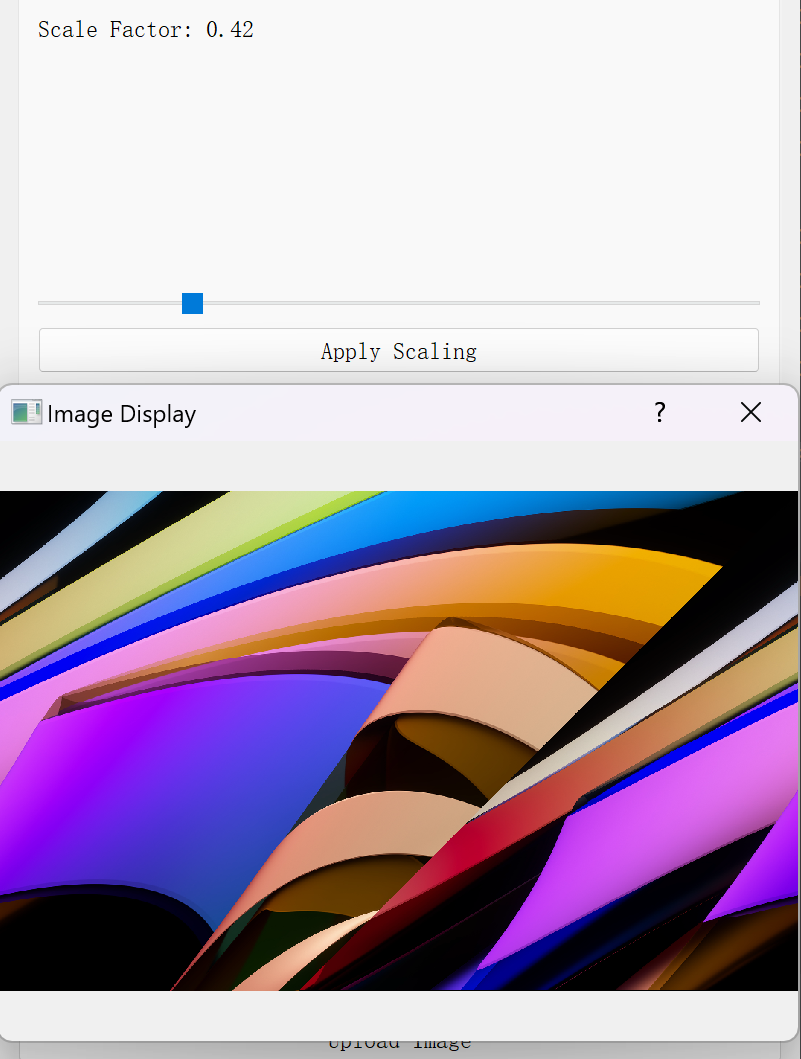
\includegraphics[width=\linewidth]{images/Design/image_processing/4/transformation1.png}
        \caption{图像缩小处理得到结果}
    \end{minipage}
    \hfill
    \begin{minipage}[b]{0.48\textwidth}
        \centering
        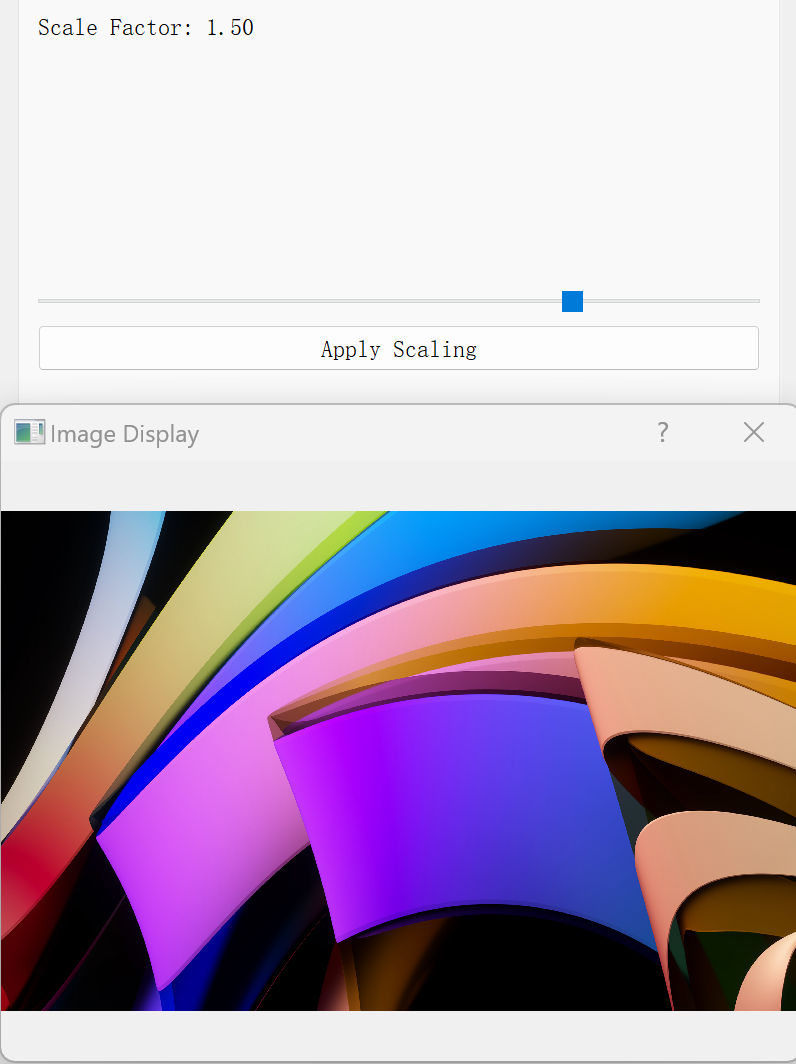
\includegraphics[width=\linewidth]{images/Design/image_processing/4/transformation2.png}
        \caption{图像放大处理得到结果}
    \end{minipage}
    
    \vspace{0.2cm}
    
    \begin{minipage}[b]{0.48\textwidth}
        \centering
        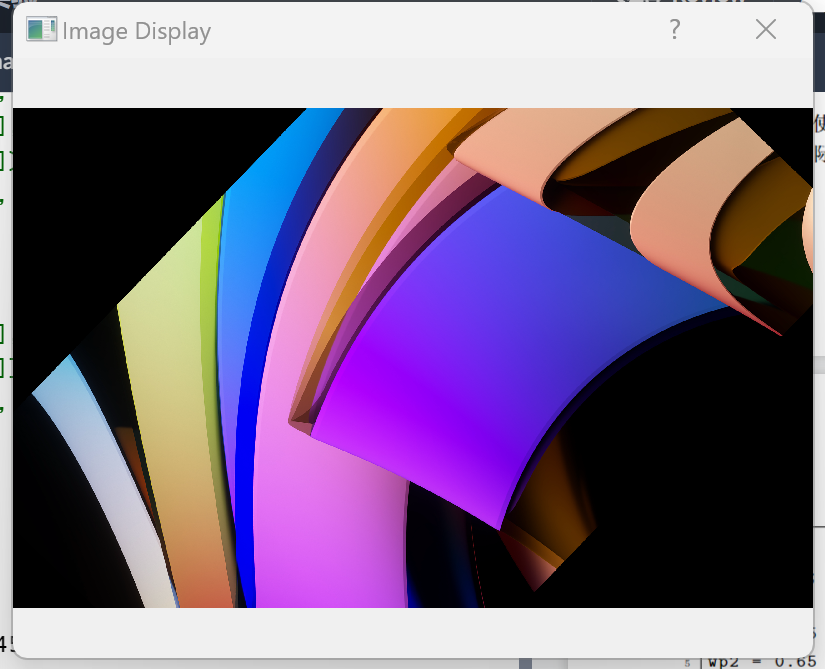
\includegraphics[width=\linewidth]{images/Design/image_processing/4/rotate1.png}
        \caption{图像旋转处理得到结果1}
    \end{minipage}
    \hfill
    \begin{minipage}[b]{0.48\textwidth}
        \centering
        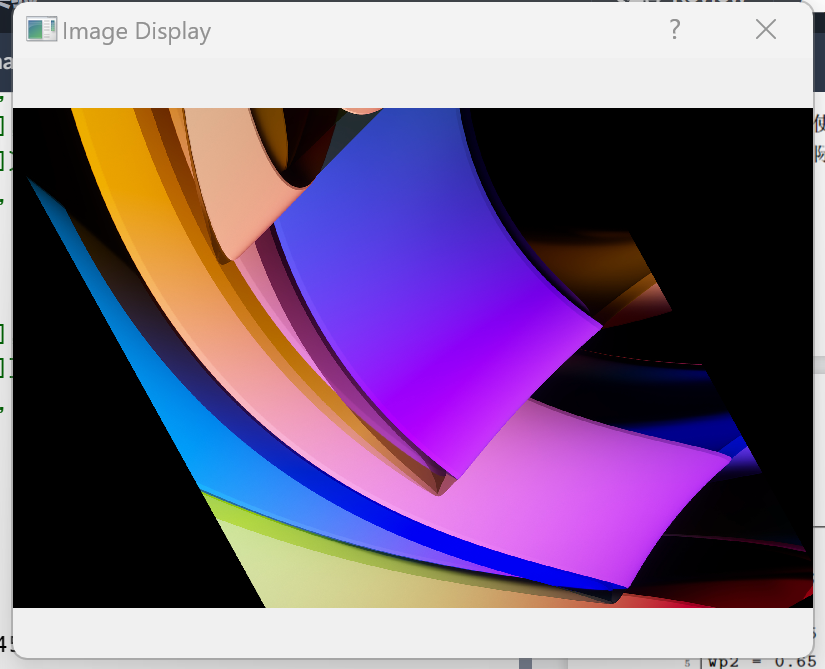
\includegraphics[width=\linewidth]{images/Design/image_processing/4/rotate2.png}
        \caption{图像旋转处理得到结果2}
    \end{minipage}
\end{figure}

图26展示了图像缩小处理的结果,图像整体被缩小,显示出原图像的全貌,但细节可能会丢失。图27展示了图像放大处理的结果,图像整体被放大,细节变得更加清晰,但可能会引入模糊或像素化问题。图28和图29分别展示了图像旋转处理的结果1和结果2,图像经过不同角度的旋转后,呈现出旋转后的视角效果。这些处理方法展示了图像几何变换的多种技术,缩放和旋转是常见的图像变换操作,应用于图像调整、对齐和视角变换等场景。

\clearpage
\subsubsection{GUI用户交互页面}
这段代码是一个使用 PyQt5 创建的图像处理应用程序的完整框架,它整合了图像卷积操作、添加噪声、应用图像效果以及图像变换等功能。下面是各部分功能的详细说明:

\begin{itemize}
    \item \textbf{类定义和初始化}
    \begin{itemize}
        \item \texttt{ImageDisplayWindow}: 一个专门用于显示处理后的图像的对话框类。它包含一个 \texttt{QLabel} 用于显示图像。
        \item \texttt{ImageProcessorApp}: 主窗口类,负责创建和管理应用程序的用户界面和功能。
    \end{itemize}

    \item \textbf{主窗口布局与控件}
    \begin{itemize}
        \item 在 \texttt{ImageProcessorApp} 的构造函数中,创建了四个标签页,分别对应不同的处理功能:卷积操作、图像处理、图像效果和图像变换。
        \item 使用 \texttt{QTabWidget} 来管理这些标签页,允许用户在不同功能间切换。
        \item 添加了一个 "Upload Image" 按钮,允许用户上传本地图像文件进行处理。
    \end{itemize}

    \item \textbf{图像上传与显示}
    \begin{itemize}
        \item \texttt{upload\_image} 方法使用 \texttt{QFileDialog} 来打开文件选择对话框,用户选择图像后,图像将被加载并转换成 RGB 格式,然后显示在 \texttt{ImageDisplayWindow} 中。
    \end{itemize}

    \item \textbf{图像处理控件的设置}
    \begin{itemize}
        \item 每个处理页 (\texttt{conv\_page}, \texttt{process\_page}, \texttt{effects\_page}, \texttt{transform\_page}) 都通过特定的方法 (\texttt{create\_convolution\_controls}, \texttt{create\_process\_controls}, \texttt{create\_effects\_controls}, \texttt{create\_transformation\_controls}) 来设置,这些方法添加具体的处理按钮和控件。
    \end{itemize}

    \item \textbf{应用滤镜的通用方法}
    \begin{itemize}
        \item \texttt{apply\_filter} 方法接受一个处理函数,应用该函数到当前加载的图像,并显示处理结果。
    \end{itemize}

    \item \textbf{运行应用}
    \begin{itemize}
        \item 在文件的最底部,创建了 \texttt{QApplication} 的实例,并显示主窗口,启动事件循环。
    \end{itemize}
\end{itemize}

这个应用程序通过图形用户界面提供了丰富的图像处理功能,用户可以通过直观的操作来查看各种图像处理效果。这不仅有助于图像处理的学习和研究,也适用于实际的图像处理任务。

\begin{lstlisting}[style=python]
from PyQt5 import QtWidgets, QtGui, QtCore
from PyQt5.QtWidgets import QMainWindow, QLabel, QTabWidget, QVBoxLayout, QPushButton, QFileDialog, QWidget, QDialog, QLineEdit
from PyQt5.QtWidgets import QSlider
from PyQt5.QtCore import Qt
import cv2
import sys

# 引入处理模块
import convolution_kernels
import image_process
import image_effects
import image_transformations

class ImageDisplayWindow(QDialog):
    def __init__(self, parent=None):
        super().__init__(parent)
        self.setWindowTitle("Image Display")
        self.setGeometry(150, 150, 800, 600)
        self.image_label = QLabel(self)
        self.image_label.resize(800, 600)
        self.image_label.setAlignment(QtCore.Qt.AlignCenter)

    def display_image(self, img):
        img = QtGui.QImage(img.data, img.shape[1], img.shape[0], QtGui.QImage.Format_RGB888).rgbSwapped()
        pixmap = QtGui.QPixmap.fromImage(img)
        self.image_label.setPixmap(pixmap.scaled(self.image_label.size(), QtCore.Qt.KeepAspectRatio))
        self.show()

class ImageProcessorApp(QMainWindow):
    def __init__(self):
        super().__init__()
        self.setWindowTitle("Image Processing App")
        self.setGeometry(100, 100, 800, 600)

        self.image_display_window = ImageDisplayWindow(self)

        self.image = None

        # 创建标签页
        tab_widget = QTabWidget(self)
        self.conv_page = QWidget()
        self.process_page = QWidget()  # 更改变量名
        self.effects_page = QWidget()
        self.transform_page = QWidget()

        tab_widget.addTab(self.conv_page, "Convolution Operations")
        tab_widget.addTab(self.process_page, "Image Process")  # 更改标签页标题
        tab_widget.addTab(self.effects_page, "Image Effects")
        tab_widget.addTab(self.transform_page, "Image Transformations")

        self.create_convolution_controls()
        self.create_process_controls()  # 更改方法名称
        self.create_effects_controls()
        self.create_transformation_controls()

        layout = QVBoxLayout()
        layout.addWidget(tab_widget)

        container = QWidget()
        container.setLayout(layout)
        self.setCentralWidget(container)

        # 添加上传图片按钮
        upload_button = QPushButton("Upload Image", self)
        upload_button.clicked.connect(self.upload_image)
        layout.addWidget(upload_button)

    def upload_image(self):
        file_name, _ = QFileDialog.getOpenFileName(self, "Open Image", "", "Image Files (*.png *.jpg *.jpeg *.bmp)")
        if file_name:
            self.image = cv2.cvtColor(cv2.imread(file_name), cv2.COLOR_BGR2RGB)
            self.image_display_window.display_image(self.image)

    def apply_filter(self, filter_func):
        if self.image is not None:
            processed_image = filter_func(self.image)
            self.image_display_window.display_image(processed_image)

    def create_convolution_controls(self):
        layout = QVBoxLayout()
        # 创建低通滤波器按钮
        lp1_button = QPushButton("Apply Lowpass Filter 1")
        lp1_button.clicked.connect(lambda: self.apply_filter(convolution_kernels.kernel_lowpass_1))
        layout.addWidget(lp1_button)

        lp2_button = QPushButton("Apply Lowpass Filter 2")
        lp2_button.clicked.connect(lambda: self.apply_filter(convolution_kernels.kernel_lowpass_2))
        layout.addWidget(lp2_button)

        lp3_button = QPushButton("Apply Lowpass Filter 3")
        lp3_button.clicked.connect(lambda: self.apply_filter(convolution_kernels.kernel_lowpass_3))
        layout.addWidget(lp3_button)

        # 创建高通滤波器按钮
        hp1_button = QPushButton("Apply Highpass Filter 1")
        hp1_button.clicked.connect(lambda: self.apply_filter(convolution_kernels.kernel_highpass_1))
        layout.addWidget(hp1_button)

        hp2_button = QPushButton("Apply Highpass Filter 2")
        hp2_button.clicked.connect(lambda: self.apply_filter(convolution_kernels.kernel_highpass_2))
        layout.addWidget(hp2_button)

        hp3_button = QPushButton("Apply Highpass Filter 3")
        hp3_button.clicked.connect(lambda: self.apply_filter(convolution_kernels.kernel_highpass_3))
        layout.addWidget(hp3_button)

        # 创建移动检测滤波器按钮
        move_horizontal_button = QPushButton("Horizontal Movement Detection")
        move_horizontal_button.clicked.connect(
            lambda: self.apply_filter(convolution_kernels.kernel_move_detection_horizontal))
        layout.addWidget(move_horizontal_button)

        move_vertical_button = QPushButton("Vertical Movement Detection")
        move_vertical_button.clicked.connect(
            lambda: self.apply_filter(convolution_kernels.kernel_move_detection_vertical))
        layout.addWidget(move_vertical_button)

        move_diagonal_button = QPushButton("Diagonal Movement Detection")
        move_diagonal_button.clicked.connect(
            lambda: self.apply_filter(convolution_kernels.kernel_move_detection_diagonal))
        layout.addWidget(move_diagonal_button)

        # 创建边缘检测按钮
        for i in range(1, 5):
            button = QPushButton(f"Apply Edge Detection {i}")
            button.clicked.connect(lambda _, k=i: self.apply_filter(getattr(convolution_kernels, f'kernel_edge_{k}')))
            layout.addWidget(button)

        # 创建梯度检测按钮
        for i in range(1, 9):
            button = QPushButton(f"Apply Gradient {i}")
            button.clicked.connect(
                lambda _, k=i: self.apply_filter(getattr(convolution_kernels, f'kernel_gradient_{k}')))
            layout.addWidget(button)

        self.conv_page.setLayout(layout)

    def create_process_controls(self):
        layout = QVBoxLayout()

        # 添加 Gaussian 噪声按钮和均值滑动条
        gauss_noise_button = QPushButton("Add Gaussian Noise")

        # 均值滑动条
        gauss_mean_slider = QSlider(Qt.Horizontal)
        gauss_mean_slider.setMinimum(-255)  # 最小值,示例为允许负均值
        gauss_mean_slider.setMaximum(255)  # 最大值
        gauss_mean_slider.setValue(0)  # 默认值为0
        gauss_mean_label = QLabel("Mean: 0")
        gauss_mean_slider.valueChanged.connect(
            lambda value: gauss_mean_label.setText(f"Mean: {value}")
        )
        layout.addWidget(gauss_mean_label)
        layout.addWidget(gauss_mean_slider)

        # 方差设置为默认值,不提供滑动条
        default_variance = 0.1  # 默认方差值

        gauss_noise_button.clicked.connect(lambda: self.apply_filter(
            lambda img: image_process.add_gaussian_noise(img, gauss_mean_slider.value(), default_variance)
        ))
        layout.addWidget(gauss_noise_button)

        # 添加 Salt and Pepper 噪声按钮和滑动条
        sp_noise_button = QPushButton("Add Salt and Pepper Noise")
        sp_amount_slider = QSlider(Qt.Horizontal)
        sp_amount_slider.setMinimum(1)
        sp_amount_slider.setMaximum(100)  # 代表比例从0.01到1.00
        sp_amount_slider.setValue(4)  # 默认值为0.04
        sp_amount_slider.valueChanged.connect(lambda value: sp_amount_label.setText(f"Amount: {value / 1000:.3f}"))
        sp_amount_label = QLabel("Amount: 0.004")
        layout.addWidget(sp_amount_label)
        layout.addWidget(sp_amount_slider)

        sp_noise_button.clicked.connect(lambda: self.apply_filter(
            lambda img: image_process.add_salt_and_pepper_noise(img, 0.5, sp_amount_slider.value() / 1000)
        ))
        layout.addWidget(sp_noise_button)

        # 添加其他图像处理操作的按钮
        self.add_other_image_processing_buttons(layout)

        self.process_page.setLayout(layout)

    def add_other_image_processing_buttons(self, layout):
        # 创建其他图像处理按钮并添加到布局
        low_pass_button = QPushButton("Apply Low Pass Filter")
        high_pass_button = QPushButton("Apply High Pass Filter")
        edge_detect_button = QPushButton("Detect Edges")
        gaussian_blur_button = QPushButton("Apply Gaussian Blur")
        sharpen_button = QPushButton("Sharpen Image")
        median_blur_button = QPushButton("Apply Median Blur")
        adjust_contrast_button = QPushButton("Adjust Contrast")

        low_pass_button.clicked.connect(lambda: self.apply_filter(image_process.apply_low_pass_filter))
        high_pass_button.clicked.connect(lambda: self.apply_filter(image_process.apply_high_pass_filter))
        edge_detect_button.clicked.connect(lambda: self.apply_filter(image_process.detect_edges))
        gaussian_blur_button.clicked.connect(
            lambda: self.apply_filter(lambda img: image_process.apply_gaussian_blur(img, 5)))
        sharpen_button.clicked.connect(lambda: self.apply_filter(image_process.sharpen_image))
        median_blur_button.clicked.connect(
            lambda: self.apply_filter(lambda img: image_process.apply_median_blur(img, 5)))
        adjust_contrast_button.clicked.connect(
            lambda: self.apply_filter(lambda img: image_process.adjust_contrast(img, 1.5)))

        layout.addWidget(low_pass_button)
        layout.addWidget(high_pass_button)
        layout.addWidget(edge_detect_button)
        layout.addWidget(gaussian_blur_button)
        layout.addWidget(sharpen_button)
        layout.addWidget(median_blur_button)
        layout.addWidget(adjust_contrast_button)

    def create_effects_controls(self):
        layout = QVBoxLayout()

        # 添加马赛克效果按钮和滑动条
        mosaic_button = QPushButton("Apply Mosaic Effect")
        mosaic_slider = QSlider(Qt.Horizontal)
        mosaic_slider.setMinimum(5)  # 最小块大小
        mosaic_slider.setMaximum(50)  # 最大块大小
        mosaic_slider.setValue(10)  # 默认块大小为 10
        mosaic_label = QLabel("Block Size: 10")
        mosaic_slider.valueChanged.connect(lambda value: mosaic_label.setText(f"Block Size: {value}"))
        mosaic_button.clicked.connect(lambda: self.apply_filter(
            lambda img: image_effects.apply_mosaic(img, mosaic_slider.value())
        ))
        layout.addWidget(mosaic_label)
        layout.addWidget(mosaic_slider)
        layout.addWidget(mosaic_button)

        # 添加晕影效果按钮和滑动条
        vignette_button = QPushButton("Apply Vignette Effect")
        vignette_slider = QSlider(Qt.Horizontal)
        vignette_slider.setMinimum(10)  # 最小强度
        vignette_slider.setMaximum(100)  # 最大强度,对应于 0.1 到 1.0 的范围
        vignette_slider.setValue(50)  # 默认强度为 0.5
        vignette_label = QLabel("Vignette Strength: 0.5")
        vignette_slider.valueChanged.connect(
            lambda value: vignette_label.setText(f"Vignette Strength: {value / 100:.2f}")
        )
        vignette_button.clicked.connect(lambda: self.apply_filter(
            lambda img: image_effects.apply_vignette(img, vignette_slider.value() / 100)
        ))
        layout.addWidget(vignette_label)
        layout.addWidget(vignette_slider)
        layout.addWidget(vignette_button)

        # 添加其他效果的按钮
        thermal_button = QPushButton("Apply Thermal Effect")
        thermal_button.clicked.connect(lambda: self.apply_filter(image_effects.apply_thermal_effect))
        layout.addWidget(thermal_button)

        sketch_button = QPushButton("Apply Sketch Effect")
        sketch_button.clicked.connect(lambda: self.apply_filter(
            lambda img: image_effects.apply_sketch_effect(img, 60, 0.07)  # 默认参数
        ))
        layout.addWidget(sketch_button)

        cartoon_button = QPushButton("Apply Cartoon Effect")
        cartoon_button.clicked.connect(lambda: self.apply_filter(image_effects.apply_cartoon_effect))
        layout.addWidget(cartoon_button)

        self.effects_page.setLayout(layout)


    def create_transformation_controls(self):
        layout = QVBoxLayout()

        # 添加缩放控制滑动条和按钮
        scale_label = QLabel("Scale Factor: 1.0", self)
        scale_slider = QSlider(Qt.Horizontal, self)
        scale_slider.setMinimum(1)
        scale_slider.setMaximum(200)  # 设定范围,例如 0.1 到 2.0 倍,内部表示为 10 到 200
        scale_slider.setValue(100)  # 默认值为 1.0,内部表示为 100
        scale_slider.valueChanged.connect(lambda value: scale_label.setText(f"Scale Factor: {value / 100:.2f}"))

        scale_button = QPushButton("Apply Scaling")
        scale_button.clicked.connect(lambda: self.apply_filter(
            lambda img: image_transformations.resize_image(img, scale_slider.value() / 100)
        ))
        layout.addWidget(scale_label)
        layout.addWidget(scale_slider)
        layout.addWidget(scale_button)

        # 添加旋转控制滑动条和按钮
        rotate_label = QLabel("Rotate Angle: 0°", self)
        rotate_slider = QSlider(Qt.Horizontal, self)
        rotate_slider.setMinimum(0)
        rotate_slider.setMaximum(360)  # 允许旋转的角度从 0 到 360 度
        rotate_slider.setValue(0)  # 默认值为 0 度
        rotate_slider.valueChanged.connect(lambda value: rotate_label.setText(f"Rotate Angle: {value}°"))

        rotate_button = QPushButton("Apply Rotation")
        rotate_button.clicked.connect(lambda: self.apply_filter(
            lambda img: image_transformations.rotate_image(img, rotate_slider.value())
        ))
        layout.addWidget(rotate_label)
        layout.addWidget(rotate_slider)
        layout.addWidget(rotate_button)

        self.transform_page.setLayout(layout)


if __name__ == "__main__":
    app = QtWidgets.QApplication(sys.argv)
    main_window = ImageProcessorApp()
    main_window.show()
    sys.exit(app.exec_())

\end{lstlisting}

\subsection{课程设计结果}
\subsubsection{GUI交互界面效果}
GUI展示效果如下:
\begin{figure}[htbp]
    \centering
    \begin{minipage}[b]{0.48\textwidth}
        \centering
        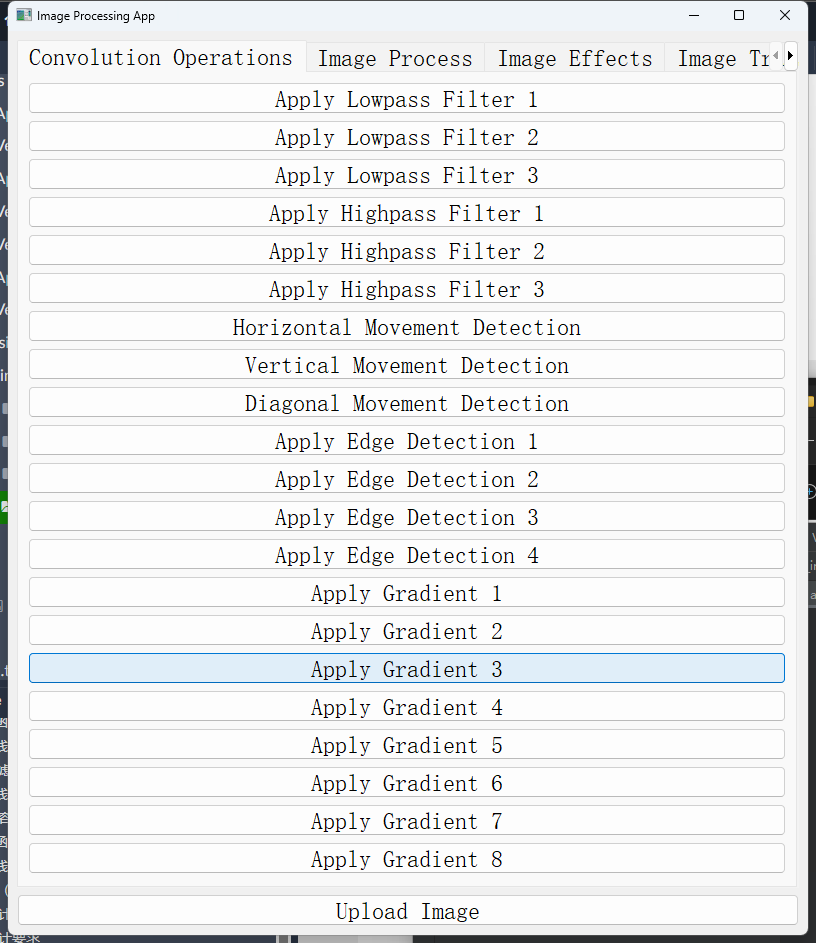
\includegraphics[width=\linewidth]{images/Design/image_processing/GUI/1.png}
        \caption{图像卷积处理选择页面}
    \end{minipage}
    \hfill
    \begin{minipage}[b]{0.48\textwidth}
        \centering
        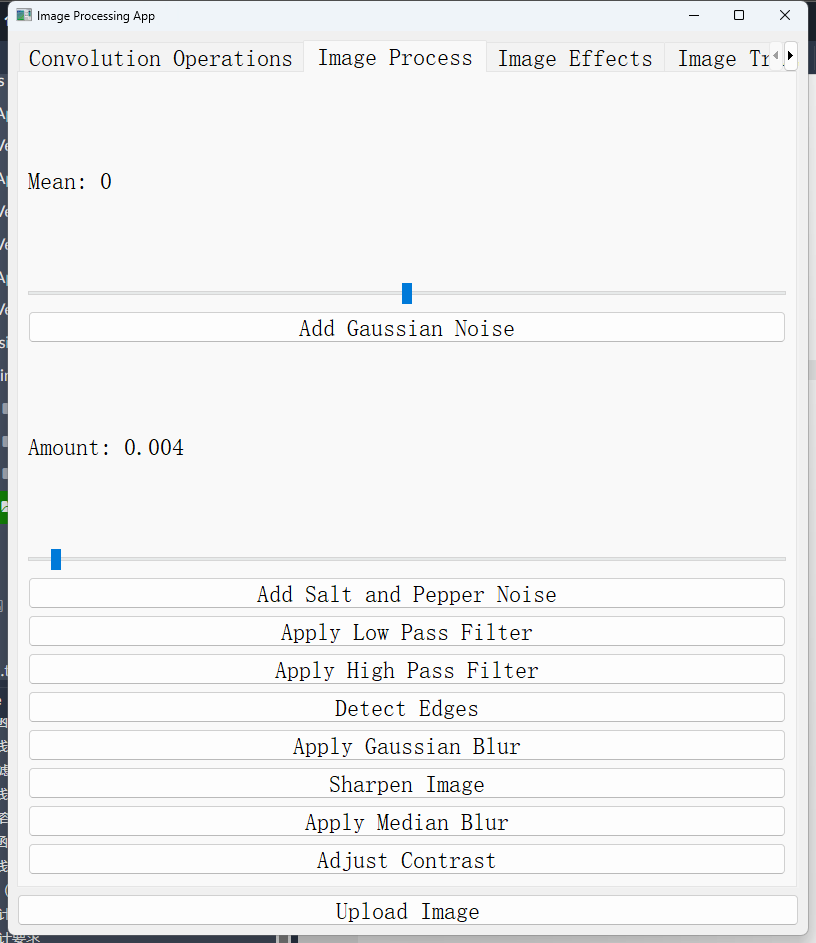
\includegraphics[width=\linewidth]{images/Design/image_processing/GUI/2.png}
        \caption{图像基本处理选择页面}
    \end{minipage}
    
    \vspace{0.2cm}
    
    \begin{minipage}[b]{0.48\textwidth}
        \centering
        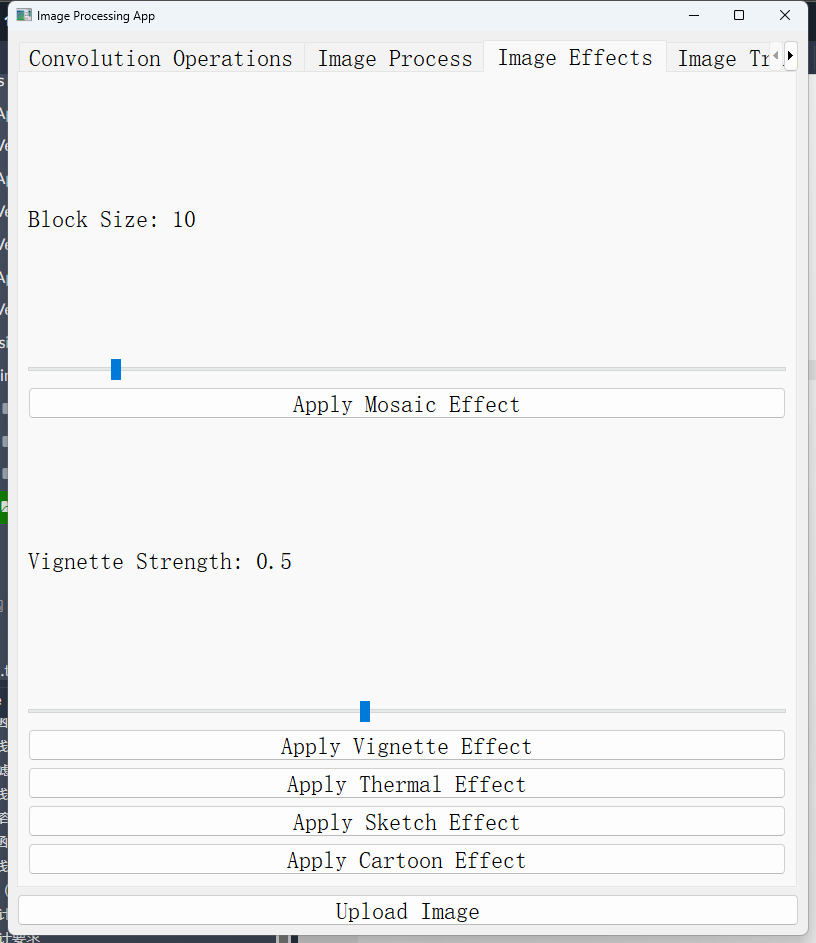
\includegraphics[width=\linewidth]{images/Design/image_processing/GUI/3.png}
        \caption{图像特效处理选择页面}
    \end{minipage}
    \hfill
    \begin{minipage}[b]{0.48\textwidth}
        \centering
        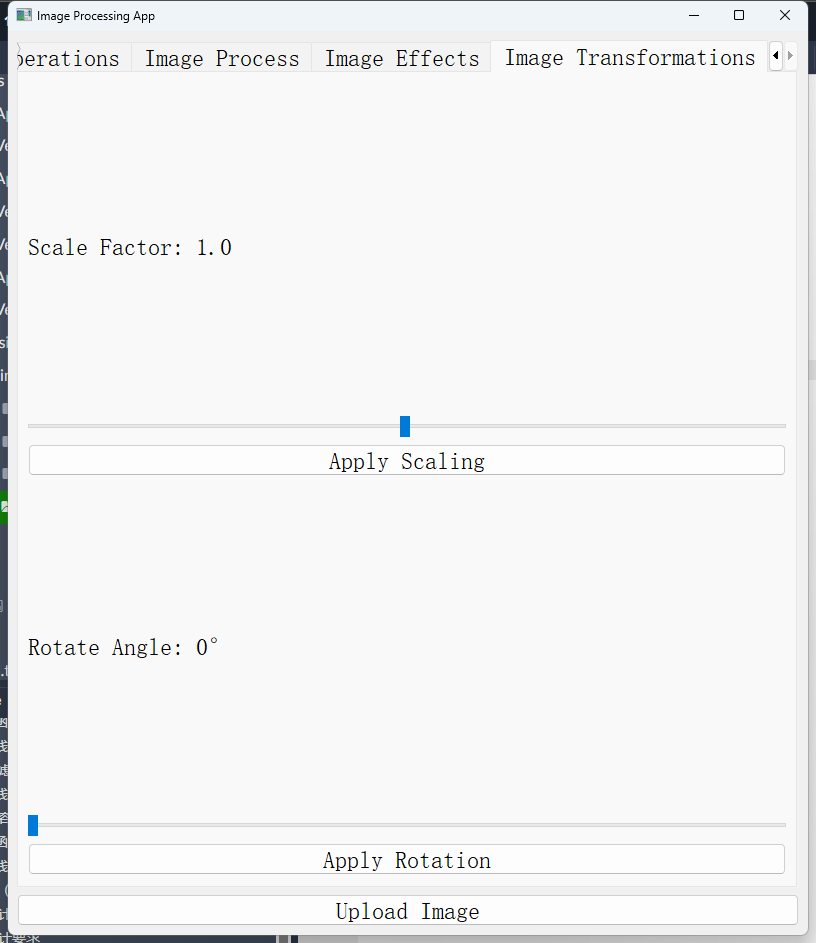
\includegraphics[width=\linewidth]{images/Design/image_processing/GUI/4.png}
        \caption{图像变换处理选择页面}
    \end{minipage}
\end{figure}

\clearpage
在点击Upload Image上传图片后,点击处理按钮(可以选择拖动滑动条来选择参数)后图片会显示在Display窗口中。
\vspace{1cm}

\centering
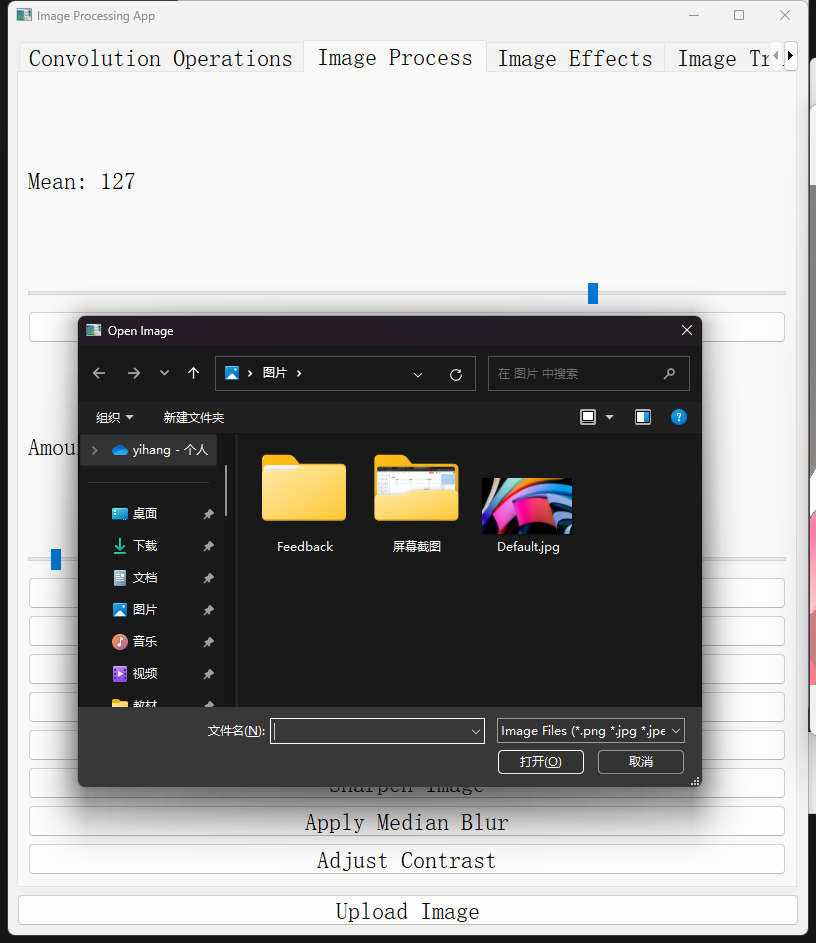
\includegraphics[width=0.6\linewidth]{images/Design/image_processing/GUI/Upload.png}
\caption{上传图片选择页面}


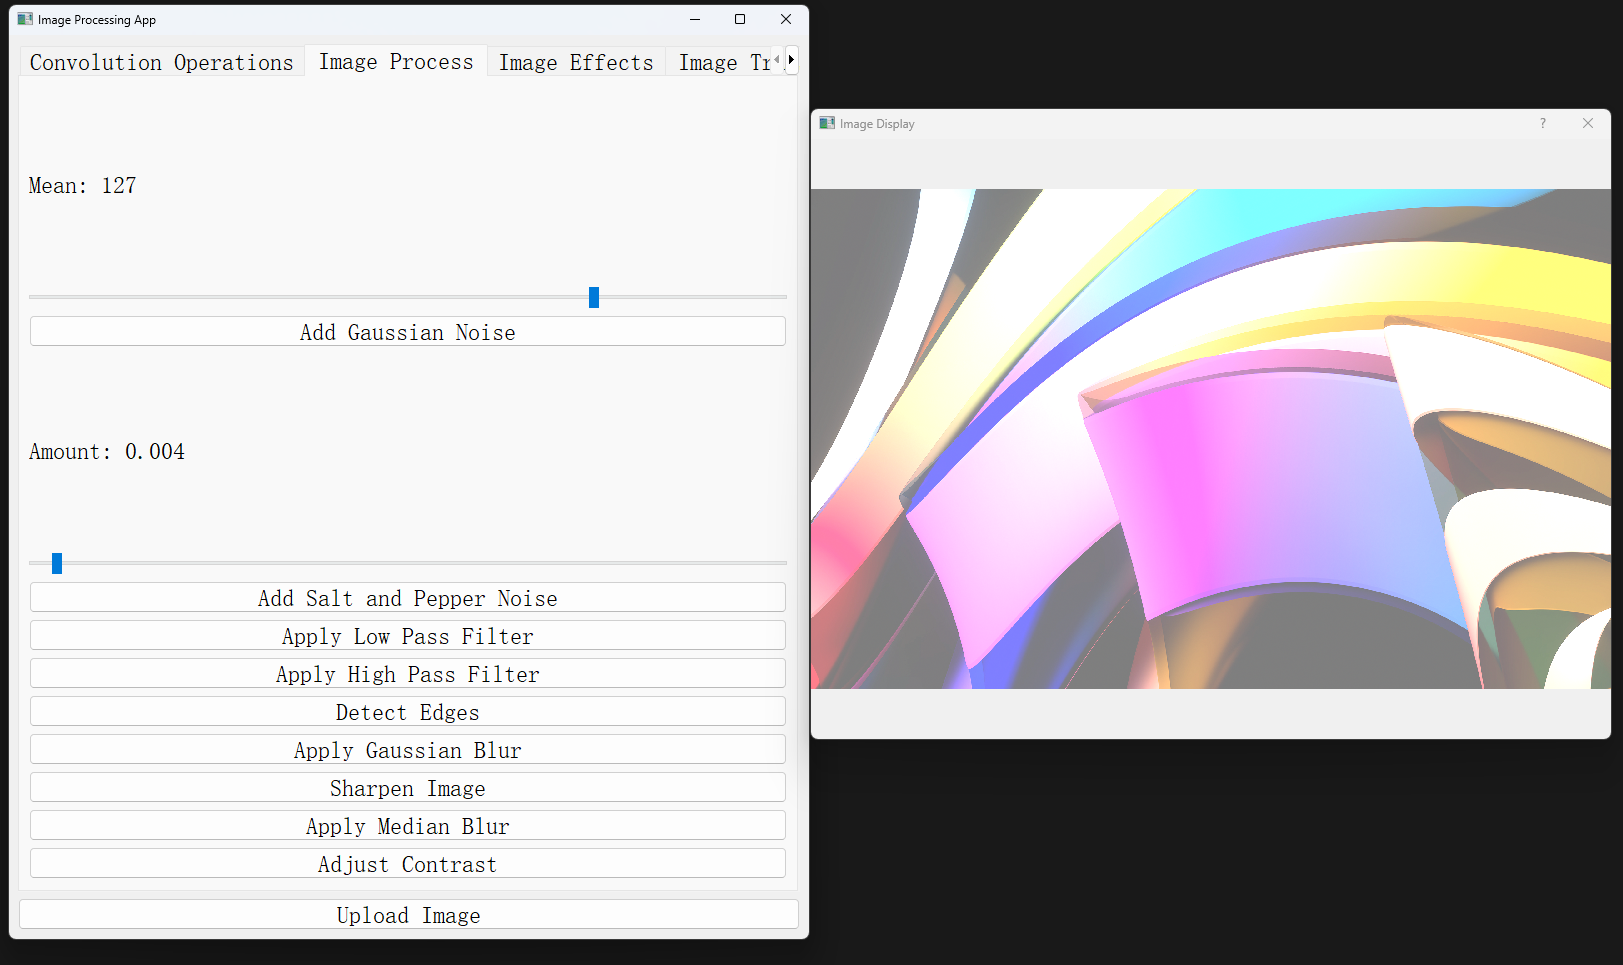
\includegraphics[width=0.8\linewidth]{images/Design/image_processing/GUI/para.png}
\caption{拖动滑动条调整函数参数传入页面}

\justifying

\newpage
\section{课程设计2(自拟):fNIRS信号的处理}
\subsection{选题背景}
\subsubsection{fNIRS信号}
功能近红外光谱(functional Near-Infrared Spectroscopy, fNIRS)是一种用于监测大脑活动的非侵入式成像技术。fNIRS通过测量大脑皮层血氧浓度的变化,反映神经活动的动态变化。当神经元活动增加时,局部的血流量和血氧水平也会相应增加,这一现象被称为血氧水平依赖(Blood Oxygen Level Dependent, BOLD)效应。fNIRS主要测量两种血红蛋白浓度的变化:氧合血红蛋白(HbO)和去氧血红蛋白(HbR)。

\subsubsection{fNIRS测量原理}
fNIRS设备通过发射近红外光(700-900纳米波长)穿透头皮和颅骨到达大脑皮层,再通过探测器接收反射光。由于HbO和HbR对近红外光的吸收率不同,可以通过分析反射光的强度变化来计算HbO和HbR的浓度变化。典型的fNIRS系统包括多个光源和探测器对,这些对以特定的排列方式放置在头皮上,覆盖感兴趣的大脑区域。

\subsubsection{应用场景}
fNIRS广泛应用于认知神经科学、心理学和医学研究中。例如,研究者可以使用fNIRS监测大脑在执行特定任务(如语言处理、注意力任务)时的活动变化,或评估不同刺激对大脑活动的影响。此外,fNIRS也用于临床诊断和康复训练,如评估脑损伤患者的功能恢复情况。

\subsection{课程设计目的}
\begin{itemize}
    \item 光密度转换:将原始光强度信号转换为光密度信号。
    \item 贝尔-兰伯特定律:应用贝尔-兰伯特定律将光密度信号转换为HbO和HbR浓度变化。
    \item 滤波处理:应用带通滤波器去除低频和高频噪声。
    \item 基线校准:对信号进行基线校准以去除基线漂移。
\end{itemize}

\subsection{课程设计原理}
\subsubsection{光密度转换}

光密度转换是指将光强度信号转换为光密度信号的过程。在近红外光谱(NIRS)测量中,光强度信号表示通过组织的光的强度。然而,这个信号受到多种因素的影响,包括组织厚度、吸收和散射等。为了更好地分析这些信号,我们通常需要将光强度信号转换为光密度信号。

光密度(Optical Density, OD)定义为光强度的对数比,公式如下:
\[
\text{OD} = \log_{10} \left( \frac{I_0}{I_t} \right)
\]
其中:
\begin{itemize}
    \item \( I_0 \) 是入射光强度。
    \item \( I_t \) 是透射光强度。
\end{itemize}

光密度的变化与血氧浓度的变化有直接关系,因为血氧饱和度会影响组织对不同波长光的吸收。因此,通过计算光密度,我们可以更准确地估计血氧浓度。

\subsubsection{血氧浓度转换}

血氧浓度转换是将光密度信号转换为氧合血红蛋白(HbO)和脱氧血红蛋白(HbR)浓度的过程。这一步骤通常使用贝尔-兰伯特定律(Beer-Lambert Law)\cite{harris2015quantitative}来完成。

贝尔-兰伯特定律描述了光在均匀介质中传播时的衰减行为。对于多重波长近红外光谱,定律可以表示为:
\[
\text{OD}(\lambda) = \epsilon_{\text{HbO}}(\lambda) \cdot C_{\text{HbO}} \cdot L + \epsilon_{\text{HbR}}(\lambda) \cdot C_{\text{HbR}} \cdot L
\]
其中:
\begin{itemize}
    \item \(\text{OD}(\lambda)\) 是波长 \(\lambda\) 处的光密度。
    \item \(\epsilon_{\text{HbO}}(\lambda)\) 和 \(\epsilon_{\text{HbR}}(\lambda)\) 分别是氧合血红蛋白和脱氧血红蛋白在波长 \(\lambda\) 处的摩尔吸收系数。
    \item \(C_{\text{HbO}}\) 和 \(C_{\text{HbR}}\) 分别是氧合血红蛋白和脱氧血红蛋白的浓度。
    \item \(L\) 是光在组织中的传播路径长度。
\end{itemize}

通过测量不同波长下的光密度,我们可以构建一个方程组来求解 \(C_{\text{HbO}}\) 和 \(C_{\text{HbR}}\)。这需要对每个波长的摩尔吸收系数进行校准和测量,并假设光传播路径长度 \(L\) 是已知的或可近似的。

\subsubsection{带通滤波处理}

带通滤波器是一种允许特定频率范围内的信号通过,同时抑制该范围之外频率成分的滤波器。对于fNIRS信号处理,带通滤波器的应用主要是为了去除不需要的噪声,同时保留有用的生理信号。

\paragraph{fNIRS信号中的频率成分}

fNIRS信号中包含多种频率成分:
\begin{itemize}
    \item \textbf{低频成分}(<0.01 Hz):通常与缓慢的生理变化(如体动、呼吸等)相关。
    \item \textbf{中频成分}(0.01 Hz - 0.1 Hz):主要反映血氧浓度变化,代表大脑活动相关的信号。
    \item \textbf{高频成分}(>0.1 Hz):通常为高频噪声,如电器噪声和高频生理噪声。
\end{itemize}

在fNIRS信号处理中,感兴趣的频率范围主要是0.01 Hz到0.1 Hz左右,因为这个范围内的信号主要反映大脑的血氧变化,是我们希望保留的有用信号。

带通滤波器通过允许特定频率范围内的信号通过,同时衰减该范围之外的信号来工作。其原理可以用以下公式表示:

\begin{equation}
y(t) = \int_{-\infty}^{\infty} x(\tau) h(t-\tau) d\tau
\end{equation}

其中:
\begin{itemize}
    \item \( y(t) \) 是滤波后的输出信号。
    \item \( x(t) \) 是输入信号(即原始fNIRS信号)。
    \item \( h(t) \) 是滤波器的冲激响应。
\end{itemize}

带通滤波器的冲激响应 \( h(t) \) 设计成只允许中频成分通过,而对低频和高频成分进行衰减。

在本设计中,带通滤波器的实现如下:

\begin{lstlisting}[language=python]
if isinstance(self.filter_para, list) \
and len(self.filter_para) >= 4 \
and isinstance(self.filter_para[0], (int, float)) \
and isinstance(self.filter_para[1], (int, float)):
    raw_haemo = raw_haemo.filter(self.filter_para[0], self.filter_para[1], 
                                 h_trans_bandwidth=self.filter_para[2], 
                                 l_trans_bandwidth=self.filter_para[3])
\end{lstlisting}

这里的滤波处理包含以下几个步骤:

\begin{enumerate}
    \item \textbf{检查滤波参数的有效性}:确保 \texttt{filter\_para} 参数是有效的,且包含了带通滤波的必要参数(下限频率、上限频率、高通带宽和低通带宽)。
    \item \textbf{应用带通滤波器}:使用 \texttt{mne} 库的 \texttt{filter} 方法对血氧浓度信号(\texttt{raw\_haemo})进行带通滤波处理。
\end{enumerate}

通过设置这些参数,带通滤波器可以有效地去除fNIRS信号中的低频和高频噪声,只保留0.01 Hz到0.1 Hz范围内的有用信号。

带通滤波的效果是去除fNIRS信号中的低频漂移和高频噪声,使得信号中的有用成分(主要是血氧浓度的变化)更加突出和清晰。这对于后续的信号分析和特征提取至关重要,因为它提高了信号的信噪比(SNR),使得我们可以更准确地检测和分析大脑活动。

\subsubsection{基线校准}

基线校准(Baseline Correction)是fNIRS信号处理中一个重要的步骤,旨在去除测量过程中由于各种原因(如仪器漂移、头皮血流变化等)导致的基线漂移。通过基线校准,可以提高信号的准确性和可靠性,使得后续的分析更加精确。

基线漂移是指在fNIRS信号中,随时间变化的慢速波动,这种波动与实际的血氧变化无关,而是由于测量过程中的各种非生理因素引起的。这些因素包括但不限于:
\begin{itemize}
    \item \textbf{仪器漂移}:由于设备本身的电子元件特性,测量信号可能会随着时间发生漂移。
    \item \textbf{头皮血流变化}:头皮和颅骨中的血流变化会影响光的吸收和散射,导致基线漂移。
    \item \textbf{环境因素}:如温度变化、光源稳定性等都会对测量结果产生影响。
\end{itemize}

基线校准的目的是通过调整信号的基线部分,使其保持在一个相对稳定的水平。通常,基线校准通过从信号中减去基线段的平均值来实现。基线段通常选择在实验开始前或特定条件下进行测量的稳定时间段。

假设我们有一个fNIRS信号 \( x(t) \),其基线段为 \( x_{\text{baseline}}(t) \),基线校准的过程可以表示为:
\begin{equation}
x_{\text{corrected}}(t) = x(t) - \bar{x}_{\text{baseline}}
\end{equation}

其中,\( \bar{x}_{\text{baseline}} \) 是基线段 \( x_{\text{baseline}}(t) \) 的平均值:
\begin{equation}
\bar{x}_{\text{baseline}} = \frac{1}{T} \int_{0}^{T} x_{\text{baseline}}(t) \, dt
\end{equation}
其中,\( T \) 是基线段的时间长度。

基线校准的步骤通常包括以下几个部分:
\begin{enumerate}
    \item \textbf{选择基线段}:在实验开始前或特定条件下进行测量的稳定时间段,选择作为基线段。
    \item \textbf{计算基线段的平均值}:对基线段进行平均,得到基线的平均值 \( \bar{x}_{\text{baseline}} \)。
    \item \textbf{校准信号}:从整个信号中减去基线段的平均值,使得校准后的信号基线部分保持在一个相对稳定的水平。
\end{enumerate}

通过基线校准,可以有效去除fNIRS信号中的基线漂移,使得信号的基线部分保持在一个相对稳定的水平。这对于后续的信号分析和特征提取非常重要,因为它提高了信号的准确性,减少了非生理因素的干扰。

基线校准前,信号中可能存在显著的慢速波动,使得信号的基线不稳定,难以准确识别实际的血氧变化。基线校准后,这些慢速波动被去除,信号的基线部分变得平稳,更容易识别和分析血氧浓度的变化。

\subsection{课程设计内容}
\subsubsection{初始化变量并读取数据}
\begin{lstlisting}[language=python]
win_ch_data = []
win_ch_sick = []
if "load_data" in self.debug_mode: print(filename) 
tag_zero, raw_intensity_arr = self.read_data_from_file(filename)
tag_table_all = self.make_tag_table_all(tag_zero)
tag_table = self.make_tag_table_conditonal(tag_zero)

\end{lstlisting}
初始化变量:win\_ch\_data和win\_ch\_sick用于存储窗口化后的数据和眩晕值。

读取数据:调用read\_data\_from\_file函数读取fNIRS数据和标签。

\subsubsection{处理为MNE对象}
\begin{lstlisting}[language=python]
info = mne.create_info(ch_names=self.ch_names, ch_types="fnirs_cw_amplitude", sfreq=self.fs, verbose=None)
for i in range(16):
    loc = np.zeros(12)
    loc[0:3] = [0, 0, 0]
    loc[9:12] = self.wavelengths[i]
    info['chs'][i]['loc'] = loc

raw_intensity = mne.io.RawArray(raw_intensity_arr.T, info, verbose=False)
raw_intensity.load_data()
montage = mne.channels.make_standard_montage('artinis-octamon')
raw_intensity.set_montage(montage)

\end{lstlisting}
创建信息对象:使用mne.create\_info创建包含通道信息的对象。

设置通道位置:为每个通道设置位置信息和波长信息。

创建Raw对象:将原始光强度数据转换为MNE的RawArray对象,并加载数据和设置空间掩膜(montage)。

\subsubsection{转换光密度与血氧密度}
\begin{lstlisting}[language=python]
raw_od = mne.preprocessing.nirs.optical_density(raw_intensity)
raw_haemo = mne.preprocessing.nirs.beer_lambert_law(raw_od, ppf=0.1)
\end{lstlisting}
光密度转换:将光强度信号转换为光密度信号。

血氧浓度转换:使用贝尔-兰伯特定律将光密度信号转换为血氧浓度信号(HbO和HbR)。

\subsubsection{制作MNE任务表并滤波}
\begin{lstlisting}[language=python]
anno_onsets, anno_durations, anno_descriptions = self.make_annotations(tag_table, data_length=len(raw_haemo))
annoatations = mne.Annotations(anno_onsets, anno_durations, anno_descriptions)
raw_haemo.set_annotations(annoatations)

if isinstance(self.filter_para, list) and len(self.filter_para) >= 4 and isinstance(self.filter_para[0], (int, float)) and isinstance(self.filter_para[1], (int, float)):
    raw_haemo = raw_haemo.filter(self.filter_para[0], self.filter_para[1], h_trans_bandwidth=self.filter_para[2], l_trans_bandwidth=self.filter_para[3])

\end{lstlisting}

制作任务表:将标签转换为MNE的注释对象,并添加到数据中。

滤波处理:应用带通滤波器去除低频和高频噪声。

\subsubsection{基线校准fNIRS信号}
\begin{lstlisting}[language=python]
def correct_baseline(self):
    if self._baseline_correct:
        print("data have been corrected!")
        return 0
    else:
        baseline_dict={}
        for sub,block,condition,win in self.win_dict.keys():
            if condition[0] == "B":
                baseline_data_source = self.win_dict[sub,block,condition,win][0]
                baseline_data = baseline_data_source.mean(axis=0)
                baseline_dict.update({(sub,block,condition[1:]):baseline_data})

        for sub,block,condition,win in self.win_dict.keys():
            if condition[0] == "B":
                continue
            source_data = self.win_dict[sub,block,condition,win][0]
            ms = self.win_dict[sub,block,condition,win][1]
            baseline_data = baseline_dict[sub,block,condition]
            corrected_data = source_data - baseline_data
            self.win_dict.update({(sub,block,condition,win):[corrected_data,ms]})
            if "correct_baseline" in self.debug_mode:
                print('baseline_data:',baseline_data)
                print('source_data:',source_data)
                print('corrected_data:',corrected_data)
        selected_keys = list(self.selected_dict.keys())
        self.selected_dict={}
        for key in selected_keys:
            self.selected_dict.update({key:self.win_dict[key][0]})
        self._baseline_correct = True
\end{lstlisting}

\subsubsection{fNIRS信号可视化展示}
\begin{lstlisting}[language=python]
import pickle
import matplotlib.pyplot as plt

# 定义加载PKL文件的函数
def load_fnirs_data(file_path):
    with open(file_path, 'rb') as file:
        data = pickle.load(file)
    return data

# 指定PKL文件路径
file_path = 'fnirs.pkl'

# 加载数据
fnirs_data = load_fnirs_data(file_path)

# 输出数据(根据实际数据结构进行处理)
print(fnirs_data)

# 打印数据的键和值的基本信息
for key, value in fnirs_data.items():
    print(f"Key: {key}")
    print(f"Array shape: {value.shape}")
    print(f"Array data (first 5 rows):\n{value[:5]}\n")

# 选择一个键进行可视化
key_to_plot = "33, 2, 'BR', 0"
data_to_plot = fnirs_data[key_to_plot]

# 绘制数据
plt.figure(figsize=(10, 6))
plt.plot(data_to_plot)
plt.title(f'Data for key: {key_to_plot}')
plt.xlabel('Sample Index')
plt.ylabel('Signal Value')
plt.legend([f'Channel {i+1}' for i in range(data_to_plot.shape[1])], loc='upper right')
plt.show()

\end{lstlisting}
\subsection{课程设计结果}
经过上述处理,我们先后可以得到以下的fNIRS信号:
\clearpage
\begin{figure}[h!]
    \centering
    \begin{minipage}[t]{0.48\textwidth}
        \centering
        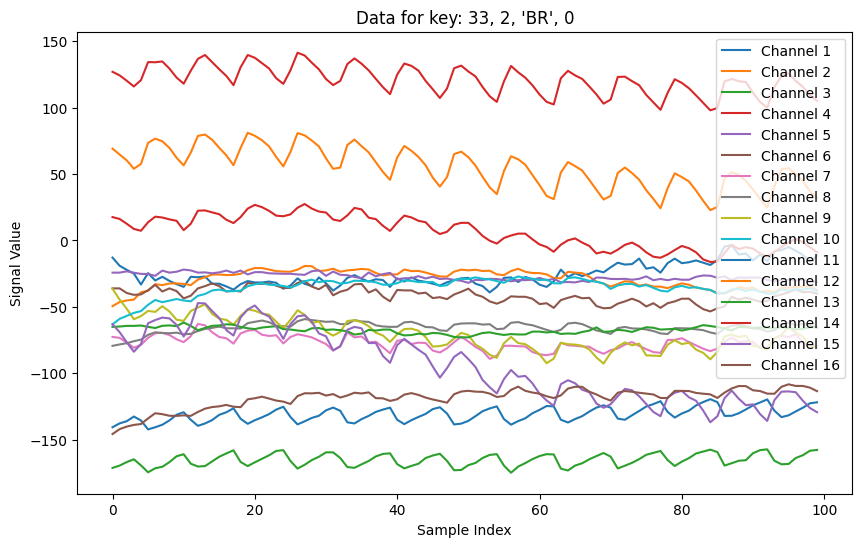
\includegraphics[width=\linewidth]{images/Design/fNIRS_processing/noprocess.png}
        \caption{无基线校准处理与带通滤波处理结果}
    \end{minipage}
    \hfill
    \begin{minipage}[t]{0.48\textwidth}
        \centering
        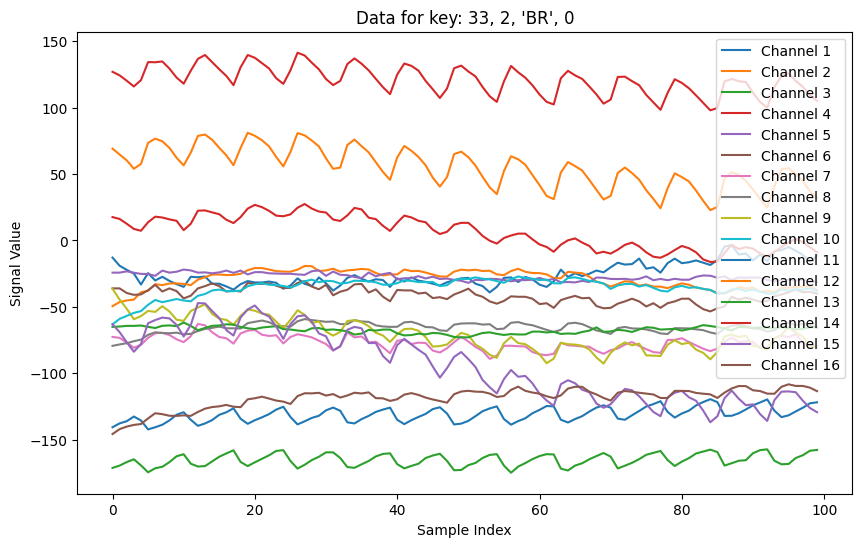
\includegraphics[width=\linewidth]{images/Design/fNIRS_processing/base_line_process.png}
        \caption{基线校准处理结果}
    \end{minipage}
\end{figure}
\vspace{0.2cm}
\begin{figure}[h!]
    \begin{minipage}[t]{0.48\textwidth}
        \centering
        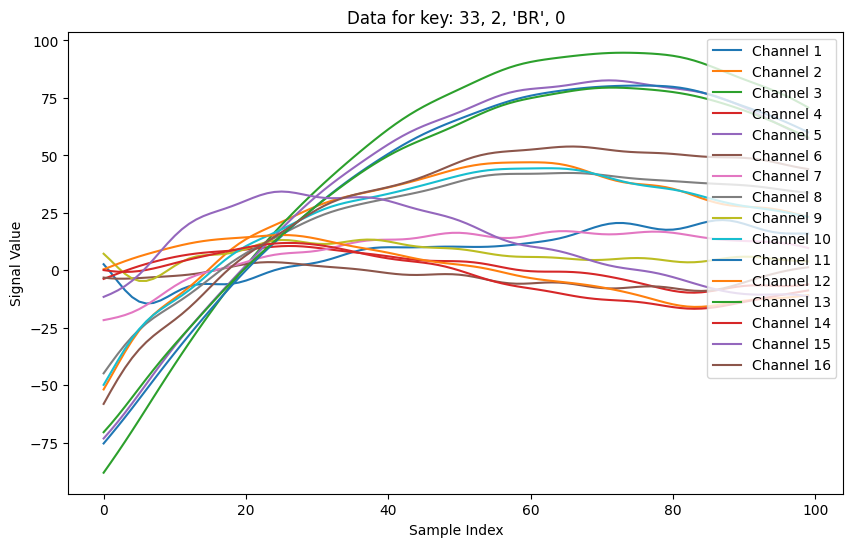
\includegraphics[width=\linewidth]{images/Design/fNIRS_processing/005-07+nobaseline.png}
        \caption{0.05-0.7Hz带通滤波处理结果}
    \end{minipage}
    \hfill
    \begin{minipage}[t]{0.48\textwidth}
        \centering
        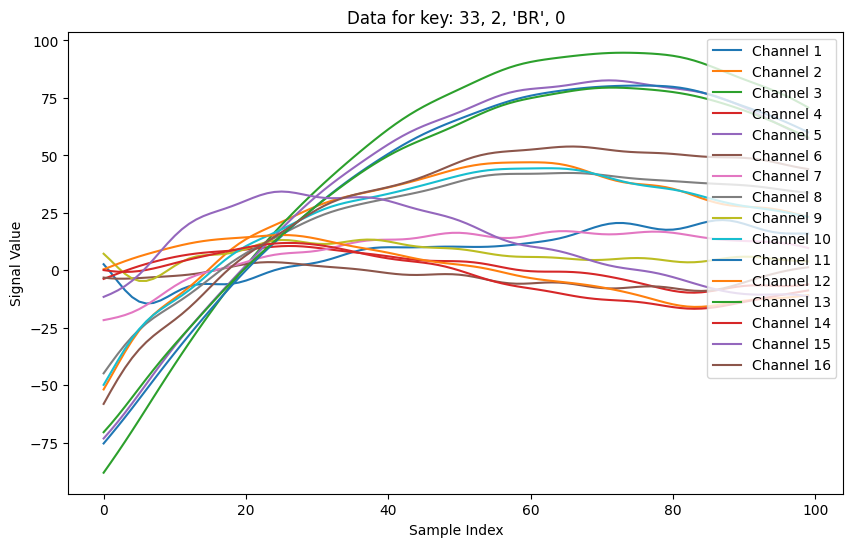
\includegraphics[width=\linewidth]{images/Design/fNIRS_processing/005-07+baseline.png}
        \caption{0.05-0.7Hz带通滤波处理+基线校准处理结果}
    \end{minipage}
\end{figure}

\clearpage
在经过了光密度转换和血氧浓度转换后,带通滤波与基线校准的处理是选择性的,需要根据后续处理要求决定。

图36展示了未经过基线校准处理的fNIRS信号。可以看到,信号中存在显著的基线漂移和噪声,难以直接用于后续分析。图37展示了经过基线校准处理后的fNIRS信号,相比未处理的信号,基线漂移被有效去除,信号的稳定性显著提高。

图38展示了应用0.05-0.7Hz带通滤波后的fNIRS信号。带通滤波器成功去除了高频和低频噪声,保留了主要的血氧变化信号。然而,仍存在一定程度的基线漂移。图39展示了在带通滤波的基础上,进一步应用基线校准处理的结果。结合两种处理方法,信号的质量得到了显著改善,基线漂移和噪声均被有效去除,信号更为平稳和清晰。

通过上述处理步骤,最终得到了质量更高的fNIRS信号。这些处理步骤包括:基线校准、带通滤波以及二者的结合应用。实验结果表明,基线校准和带通滤波的联合应用可以显著提高fNIRS信号的质量,为后续的信号分析和特征提取提供了可靠的数据基础。

\newpage
\section{鸣谢}
在完成本次实验和论文的过程中,我深深感受到教师的指导对于学生成长的重要性。在此,我要特别感谢我的数字信号处理老师宁更新老师。他在整个教学和指导过程中表现出的敬业精神和无私奉献令我深受感动。

宁老师不仅在课堂上为我们详细讲解了数字信号处理的基本原理和技术,还在实验过程中给予了我大量的指导和帮助。无论是遇到理论上的困惑还是实验中的难题,他总是耐心地解答,帮助我逐步理解和解决问题。宁老师严谨的科研态度和一丝不苟的工作作风,让我学到了如何在科研中保持专注和细致。

通过宁老师的教导,我不仅掌握了许多专业知识,更学会了如何进行科学研究,如何设计和执行实验,以及如何分析和解释实验结果。这些宝贵的经验和知识将对我未来的学习和科研道路产生深远的影响。

宁老师的鼓励和支持也给予了我极大的动力,使我在面对困难时能够坚持不懈,不断进步。他的学术造诣和高尚的师德,将成为我未来学习和工作的榜样和指引。

再次衷心感谢宁更新老师的辛勤付出和无私帮助!他的教诲将伴随我在今后的学习和科研道路上不断前行。
\newpage
\bibliographystyle{unsrt}
\bibliography{bibliography/exp2}

\end{document}

